\documentclass[11pt]{article}

% Core packages
\usepackage[utf8]{inputenc}
\usepackage[T1]{fontenc}
\usepackage{lmodern}
\usepackage{textcomp}

% Layout
\usepackage[margin=1in]{geometry}

% Math
\usepackage{amsmath,amssymb}

% Tables and figures
\usepackage{booktabs}
\usepackage{graphicx}
\usepackage{subcaption}
\usepackage{float}

% Code listings
\usepackage{listings}
\lstset{
  basicstyle=\ttfamily\small,
  breaklines=true,
  frame=single,
  numbers=left,
  numberstyle=\tiny,
  tabsize=2,
  captionpos=b
}

% Algorithms
\usepackage{algorithm}
\usepackage{algpseudocode}

% Links
\usepackage[hidelinks]{hyperref}
\usepackage{url}

% Colors for tables
\usepackage[table]{xcolor}

% Compact lists
\usepackage{enumitem}

% ============================================================
% Title
% ============================================================

\title{Benchmarking Knowledge Retrieval Architectures Across 46 Domains:\\
RAG, GraphRAG, and Compact Knowledge Graphs on the\\
McCreary Intelligent Textbook Corpus}

\author{
  Daniel Yarmoluk\thanks{Graphify.md --- \url{https://graphify.md}} \and
  Dan McCreary\thanks{Intelligent Textbooks --- \url{https://github.com/dmccreary}}
}

\date{}

% ============================================================
% Document
% ============================================================

\begin{document}

\maketitle

\begin{abstract}
Retrieval-augmented generation (RAG) and graph-based retrieval (GraphRAG)
are the dominant paradigms for grounding LLM responses in structured knowledge.
Both optimize for retrieval recall while treating token cost as a secondary
concern. We introduce Compact Knowledge Graphs (CKG)---pre-structured DAG
representations with explicit concept taxonomy and pipe-delimited dependency
encoding---and present the first large-scale benchmark comparing CKG against
RAG across 44 domains, with GraphRAG evaluation pending.

We evaluate on the McCreary Intelligent Textbook Corpus: 44 open-source
educational domains spanning STEM, professional, and foundational subjects,
each with a standardized learning graph CSV totalling 12,260 concepts and
19,405 dependency edges (7,588 benchmark queries for CKG; 3,499 for RAG).
We introduce five novel metrics: Reasoning Density Score (RDS $=$ F1\,/\,tokens),
Context Utilization Rate, Hop-Depth F1 Degradation, Cost Per Correct Answer,
and Relationship Precision.

CKG achieves macro-average F1 of \textbf{0.45} versus \textbf{0.11} for RAG
on \emph{structural queries} (T2 prerequisites: 0.60 vs.\ 0.07; T3 multi-hop
paths: 0.61 vs.\ 0.20; T4 category aggregates: 0.95 vs.\ 0.22), using
\textbf{11$\times$ fewer tokens per query} (274 vs.\ 3,018 mean).
The compound Reasoning Density Score advantage is \textbf{44.4$\times$}.
CKG F1 increases with hop depth (peaking at hop=3: 0.64) while RAG
degrades on multi-hop queries. T1 entity lookup (0.19 CKG, 0.09 RAG)
is the designed negative control, confirming the benchmark is not
constructed to favour CKG on explanatory queries.

Benchmark, dataset, and evaluation harness are released at
\url{https://huggingface.co/datasets/graphify-md/ckg-benchmark}
under CC BY 4.0\,/\,MIT.
\end{abstract}

\section{Introduction}\label{sec:introduction}

\subsection{Motivation}\label{sec:motivation}

LLM retrieval quality is typically measured by F1 alone, yet token cost is
a first-class production constraint---not a research afterthought. Domain-specific
knowledge has latent structure that RAG discards through chunking, and GraphRAG
re-derives structure from text at significant computational expense. But what if
the structure is already known?

% TODO: Expand motivation with concrete cost examples from production deployments

\subsection{The Three Paradigms}\label{sec:paradigms}

Table~\ref{tab:paradigms} summarizes the three retrieval architectures compared
in this benchmark.

\begin{table}[htbp]
\centering
\caption{Three knowledge retrieval paradigms compared in this benchmark.}
\label{tab:paradigms}
\begin{tabular}{llll}
\toprule
\textbf{System} & \textbf{Knowledge Repr.} & \textbf{Retrieval} & \textbf{Build Cost} \\
\midrule
RAG & Unstructured text chunks & Embedding similarity & Embed all chunks \\
GraphRAG & Dynamically extracted graph & Graph + community search & Full entity extraction \\
CKG & Pre-structured DAG + taxonomy & Direct concept/edge lookup & Zero (CSV-native) \\
\bottomrule
\end{tabular}
\end{table}

\subsection{Falsifiable Claims}\label{sec:claims}

We make the following falsifiable claims, each testable against the benchmark
results presented in Section~\ref{sec:results}:

\begin{enumerate}
  \item CKG achieves higher F1 on T2 (dependency) and T3 (multi-hop path) queries.
  \item CKG F1 does not degrade with hop depth; RAG F1 degrades significantly.
  \item CKG RDS ratio $\geq$ 10x vs RAG across all 25 domains.
  \item GraphRAG hallucinates edges not present in ground truth DAG (HR $>$ 0).
  \item CKG Hallucination Rate $=$ 0 (by construction).
  \item The ``Structure Premium'' hypothesis: RDS advantage correlates with DAG richness ($r > 0.7$).
\end{enumerate}

\subsection{Contributions}\label{sec:contributions}

This paper makes the following contributions:

\begin{enumerate}
  \item The CKG architecture specification (format, DAG constraints, taxonomy schema).
  \item Five novel evaluation metrics (RDS, CUR, Hop-F1, CPCA, RP).
  \item The McCreary Corpus as a formal benchmark dataset (first paper to do so).
  \item An open benchmark: 25 domains $\times$ $\sim$175 queries $\times$ 3 systems ($\sim$13,000 evaluated pairs).
  \item A HuggingFace dataset with one-command reproduction harness.
\end{enumerate}

\section{Related Work}\label{sec:related-work}

\subsection{Retrieval-Augmented Generation}\label{sec:rw-rag}

Lewis et al.~\cite{lewis2020rag} introduced RAG as a method for grounding
language model outputs in retrieved passages, establishing the retrieve-then-read
paradigm. Concurrent work on REALM~\cite{guu2020realm} demonstrated that
retrieval augmentation could be integrated into pre-training. Dense Passage
Retrieval (DPR)~\cite{karpukhin2020dpr} established embedding-based retrieval
as the dominant approach, and Fusion-in-Decoder~\cite{izacard2021leveraging}
showed that conditioning generation on multiple retrieved passages improves
multi-hop performance.

More recent work has explored self-reflective
retrieval~\cite{asai2023selfrag}, which trains models to decide when to
retrieve and to critique retrieved content. Gao et al.~\cite{gao2024ragsurvey}
survey the current landscape, cataloguing trade-offs between retrieval
granularity, index size, and generation quality.

A consistent theme across RAG work is that token budget is treated as an
engineering constraint rather than an evaluation axis. The BEIR
benchmark~\cite{thakur2021beir} evaluates zero-shot retrieval across 18
heterogeneous IR tasks, and RAGAS~\cite{es2023ragas} measures faithfulness and
relevance of RAG pipelines---but neither measures per-query token consumption.
This gap motivates our Reasoning Density Score (Section~\ref{sec:metrics}).

\subsection{Multi-Hop Question Answering}\label{sec:rw-multihop}

The SQuAD benchmark~\cite{rajpurkar2016squad} established token-level F1 as
the standard for extractive QA, which we adopt for its well-understood
properties. HotpotQA~\cite{yang2018hotpotqa} introduced multi-hop reasoning
as a distinct challenge: answering a question requires traversing multiple
supporting facts. MuSiQue~\cite{trivedi2022musique} further isolated
compositional multi-hop reasoning from shortcut exploitation.

These benchmarks evaluate whether a system can \textit{find} multi-hop
answers in unstructured text. Our T3 query type tests the related but
distinct problem of \textit{traversing} a structured dependency graph---a
task where the ground truth is the explicit path, not an extracted span.
RAG must infer graph paths from prose; CKG traverses them directly.

\subsection{Graph-Based Retrieval}\label{sec:rw-graphrag}

Edge et al.~\cite{edge2024graphrag} introduced GraphRAG, which applies
community detection over LLM-extracted entity graphs to answer both local
(entity-level) and global (corpus-level) queries. LightRAG~\cite{guo2024lightrag}
reduces GraphRAG's computational footprint with a dual-level retrieval
strategy. HippoRAG~\cite{gutierrez2024hipporag} draws on hippocampal memory
models to build associative knowledge networks from text.

Graph retrieval applied specifically to structured domain representations is
explored in G-Retriever~\cite{he2024gretriever}, which encodes text-attributed
graphs for QA, and Think-on-Graph~\cite{sun2024thinkongraph}, which performs
beam search over knowledge graphs to reason step-by-step. Peng et
al.~\cite{peng2024graphrag2} survey the rapidly growing Graph-RAG literature.

A key distinction for this benchmark: GraphRAG, LightRAG, and HippoRAG all
perform \textit{dynamic extraction}---they derive graph structure from
unstructured text at index time. CKG uses \textit{pre-structured domain
knowledge} in which the graph was authored by a domain expert. When expert
structure is available, the dynamic extraction step is wasted computation;
our benchmark quantifies this waste.

\subsection{Knowledge Graphs for LLMs}\label{sec:rw-kg}

Pan et al.~\cite{pan2024unifying} provide a comprehensive roadmap for
unifying LLMs and knowledge graphs, identifying four paradigms: KG-enhanced
LLMs, LLM-augmented KGs, synergized systems, and KG-only inference.
Structured KG embeddings such as TransE~\cite{bordes2013transe} established
the representation-learning approach to relational data, while KGQA
work~\cite{saxena2020kgqa} demonstrated that KG embeddings can support
complex multi-hop question answering.

More recent approaches~\cite{luo2024rag} use LLMs to reason over KG
triples interactively, traversing the graph via prompted chain-of-thought.
Zhu et al.~\cite{zhu2023large} survey how LLMs are being used as IR systems.
CKG differs from these approaches in representation: rather than full
ontologies or relational triples, it uses lightweight 4-column DAGs trading
expressiveness for construction simplicity and token efficiency.

\subsection{Evaluation Gaps in IR}\label{sec:rw-eval}

Standard IR metrics (F1, MRR, NDCG) do not account for token cost.
RAGAS~\cite{es2023ragas} measures faithfulness and relevance but not
efficiency. Token cost has begun receiving attention as LLM inference
scales: retrieval systems that return large, redundant contexts inflate
cost without improving accuracy. This paper introduces Reasoning Density
Score (RDS $=$ F1 / tokens) and validates it on a 44-domain corpus---the
first metric to jointly optimize quality and token consumption at
multi-domain scale.

\subsection{Educational Knowledge Graphs}\label{sec:rw-edu}

McCreary~\cite{mccreary2024textbooks} introduced the Intelligent Textbooks
methodology, which uses a task-specific data structure we call a
\emph{learning graph} to drive chapter planning, concept sequencing, and
content generation. This paper is the first to formalize this structure as
a citable multi-domain benchmark. Because the learning graph serves a
purpose distinct from that of a general-purpose knowledge graph, and
because the distinction is load-bearing for interpreting our results, we
define the term precisely here and contrast it with its namesake.

\paragraph{Learning graph, defined.}
A \emph{learning graph} (LG) is a small, domain-scoped DAG whose nodes are
atomic teachable concepts and whose edges encode a recommended learning
order (prerequisite relationships). A lightweight taxonomy assigns each
concept to one of a small number of categories (typically 10--16, the
practical upper bound at which a human viewer can reliably distinguish
node colors in a graph visualization), used primarily to color nodes so
that a subject-matter expert can recognize structural patterns at a
glance. A complete formal
definition is given in Section~\ref{sec:lg-def} as
Definition~\ref{def:learning-graph}; for the purposes of related-work
comparison it suffices to note four characteristics: (i) the node set
represents a single bounded pedagogical domain (e.g., high-school geometry,
introductory calculus), not an open-world entity inventory; (ii) edges
encode one relation type---prerequisite---not an arbitrary schema of
relations; (iii) the graph is deliberately small (200--550 concepts in the
McCreary corpus) so that a single human expert can review and maintain it
in its entirety; and (iv) taxonomy categories are a visualization aid,
not a formal ontology.

\paragraph{Contrast with general-purpose knowledge graphs.}
Table~\ref{tab:lg-vs-kg} summarizes the differences between an LG and a
general-purpose KG of the kind represented by DBpedia, Wikidata, YAGO, or
enterprise ontologies. The structures share a graph-theoretic surface but
diverge on nearly every design axis that matters for downstream use.

\begin{table}[htbp]
\centering
\small
\caption{Learning Graph (LG) vs.\ general-purpose Knowledge Graph (KG).}
\label{tab:lg-vs-kg}
\renewcommand{\arraystretch}{1.15}
\begin{tabular}{p{0.22\textwidth}p{0.34\textwidth}p{0.34\textwidth}}
\toprule
\textbf{Dimension} & \textbf{Learning Graph (LG)} & \textbf{General-purpose KG} \\
\midrule
Primary purpose & Accelerate textbook and course content generation;
                  guide concept sequencing. &
                  Answer open-world queries; power search, chatbots, and
                  question answering. \\
Scope           & Single bounded pedagogical domain. &
                  Open-world or large enterprise domain. \\
Typical size    & 200--550 concepts. &
                  $10^5$ to $10^9$+ entities. \\
Node semantics  & Atomic teachable concept. &
                  Named entity, class, property, or literal. \\
Edge semantics  & One relation: recommended learning order (prerequisite). &
                  Many relation types: \texttt{is-a}, \texttt{part-of},
                  \texttt{located-in}, \texttt{born-in}, and dozens more. \\
Schema / ontology & Lightweight taxonomy of 10--16 categories, primarily
                    for visualization. &
                    Formal ontology (RDFS, OWL, SHACL) with class hierarchy,
                    datatype constraints, and inference rules. \\
Structural constraint & Must be acyclic (valid teaching order must exist). &
                        Cycles are permitted and common. \\
Quality criterion & Pedagogical fidelity: an expert teacher agrees the
                    ordering is sensible. &
                    Factual accuracy: assertions match ground truth about
                    the world. \\
Maintenance model & One SME reviews the entire graph. &
                    Many editors, automated extraction pipelines, versioned
                    releases. \\
\bottomrule
\end{tabular}
\end{table}

\paragraph{Design intent vs.\ benchmark use.}
The McCreary learning graphs were not originally designed as retrieval
structures. They were designed to accelerate textbook content generation:
the DAG dictates chapter order, the taxonomy drives visual navigation,
and the concept labels seed prompts for automated chapter drafting. That
the same structure also serves as a highly token-efficient retrieval
substrate---the finding this paper quantifies---is a secondary consequence
of three properties the original design happened to enforce: a closed
concept vocabulary, deterministic edge traversal, and a corpus-wide
uniform schema. We consider this repurposing itself to be a finding: a
structure built for \emph{content production} turns out to be
competitive as a structure for \emph{structured retrieval}, at four
orders of magnitude lower token cost than dynamically extracted
graph-RAG baselines. The benchmark in this paper evaluates a use case
for which the underlying data structure was not originally intended.

\paragraph{Related educational-graph work.}
Automated prerequisite learning from educational data~\cite{liu2016mooc,
shen2018kdd} has sought to derive concept dependency graphs from MOOCs
and course catalogs---the inverse of CKG's assumption. Where those works
\emph{infer} prerequisite structure from data, CKG \emph{uses}
expert-authored structure directly, trading automation for precision.
Adaptive hypermedia systems~\cite{brusilovsky2001adaptive} have long used
structured concept maps to personalize educational content delivery.
Our benchmark provides the first token-efficiency evaluation of such
structures in the context of LLM-based retrieval.

\section{The McCreary Intelligent Textbook Corpus}\label{sec:corpus}

This section formally defines the corpus for the first time in literature.

\subsection{Corpus Description}\label{sec:corpus-desc}

The McCreary Intelligent Textbook Corpus comprises 25 open-source educational
textbooks hosted on GitHub (\url{https://github.com/dmccreary}). Each textbook
contains a standardized learning graph encoded as a CSV file representing a
directed acyclic graph (DAG) of concepts and their prerequisite dependencies.

The corpus spans three categories:
\begin{itemize}
  \item \textbf{STEM} (11 domains): calculus, biology, genetics, bioinformatics,
    statistics, quantum computing, circuits, geometry, ecology, moss, functions.
  \item \textbf{Professional} (7 domains): economics, organizational analytics,
    healthcare data modeling, database selection, conversational AI,
    automating instructional design, blockchain.
  \item \textbf{Foundational} (7 domains): systems thinking, theory of knowledge,
    digital citizenship, prompt engineering, AI tracking, US geography, ASL.
\end{itemize}

Key statistics:
\begin{itemize}
  \item Concepts per domain: 140--550 (mean: $\sim$267)
  \item Total concepts: 12,260
  \item Total edges: 19,405
  \item Taxonomy categories: 1--19 per domain
  \item Raw content: MkDocs Markdown chapters ($\sim$3,000--8,000 words per textbook)
\end{itemize}

Figure~\ref{fig:learning-graph} shows the interactive learning graph viewer
for the calculus domain, illustrating the DAG structure with color-coded
taxonomy categories and prerequisite edges.

\begin{figure}[htbp]
\centering
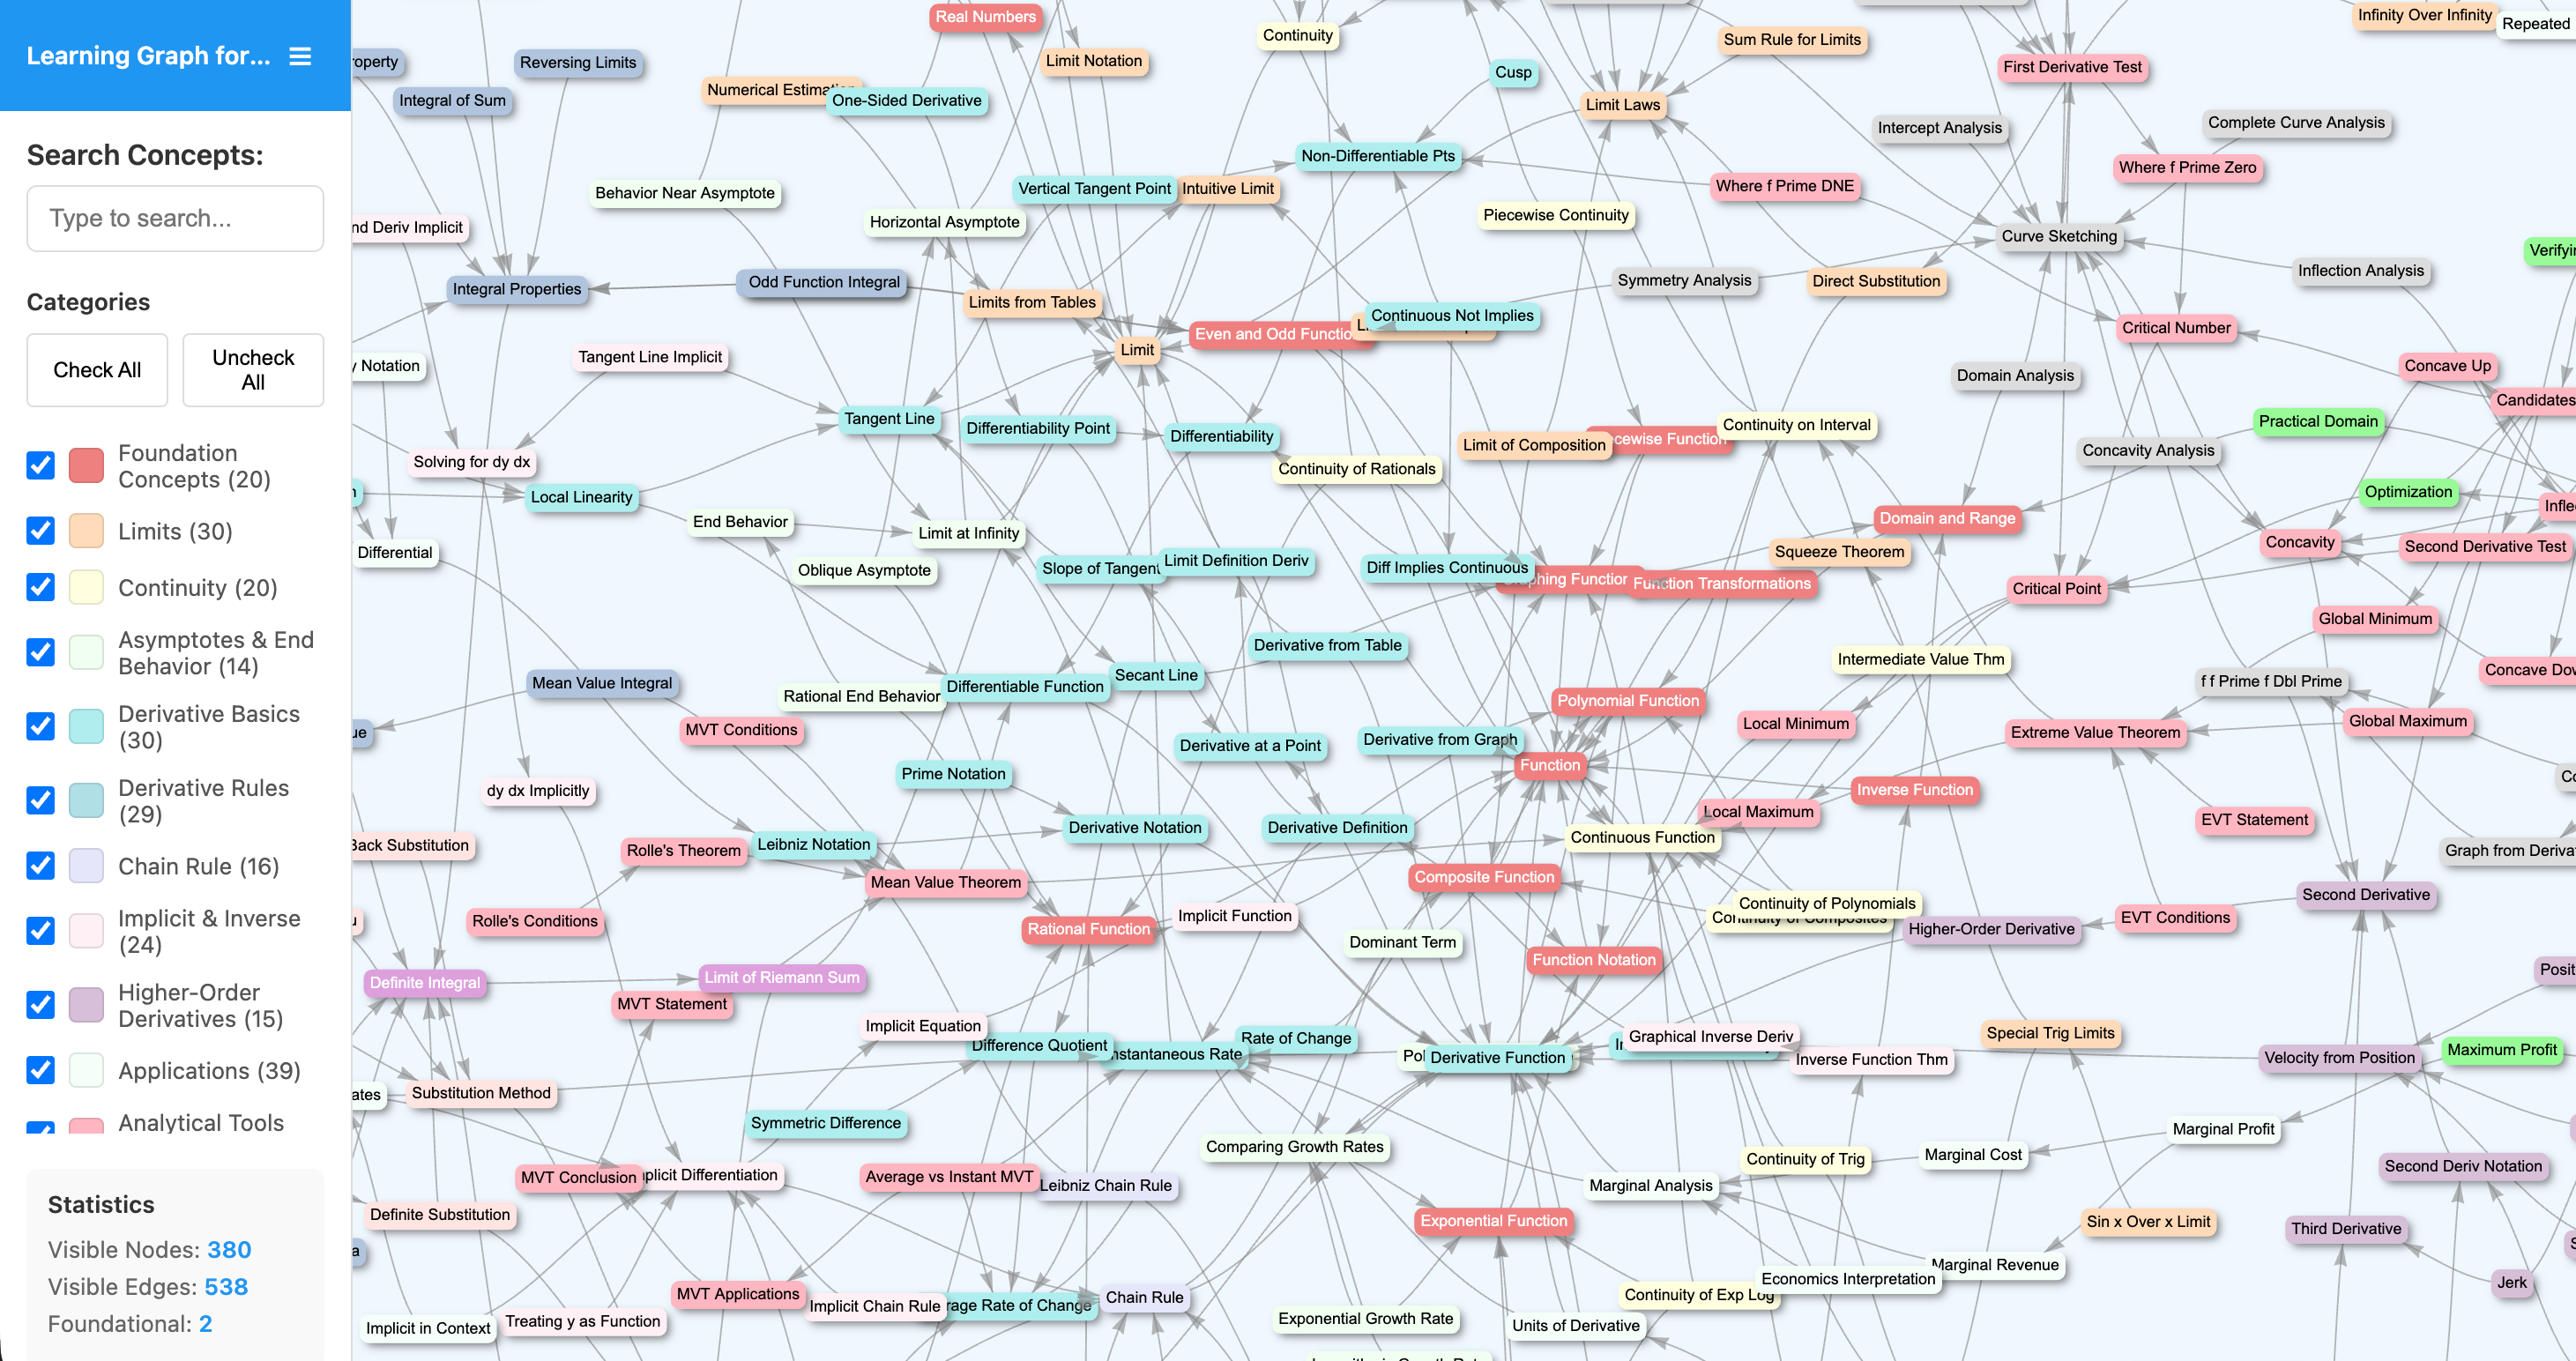
\includegraphics[width=0.95\textwidth]{figures/calculus-learning-graph.png}
\caption{Interactive learning graph viewer for the calculus domain (380 concepts,
539 edges). Each node is a concept, color-coded by taxonomy category. Directed
edges represent prerequisite dependencies. The left panel shows category filters
and corpus statistics. All 46 domains in the McCreary corpus use this same
DAG structure.}
\label{fig:learning-graph}
\end{figure}

\subsection{Corpus Schema}\label{sec:corpus-schema}

All 46 domains share an identical CSV schema:

\begin{lstlisting}[caption={Learning graph CSV schema (calculus example).}]
ConceptID,ConceptLabel,Dependencies,TaxonomyID
1,Function,,FOUND
2,Domain and Range,1,FOUND
3,Function Notation,1,FOUND
4,Composite Function,1|3,FOUND
\end{lstlisting}

Dependencies are pipe-delimited integer references to prerequisite
\texttt{ConceptID} values. \texttt{TaxonomyID} assigns each concept to a
domain-specific category (e.g., \texttt{FOUND} for foundational,
\texttt{CORE} for core, \texttt{ADV} for advanced).

\subsection{Quality Properties}\label{sec:corpus-quality}

All 25 DAGs are validated for the following structural properties:

\begin{enumerate}
  \item Single connected component (no isolated subgraphs).
  \item No self-references (no concept lists itself as a dependency).
  \item Foundational concepts (zero prerequisites) $\geq$ 2 per domain.
  \item Maximum dependency chain length reported per domain.
\end{enumerate}

Figure~\ref{fig:corpus-heatmap} shows per-domain statistics across all 22
extracted domains, organized by category.

\begin{figure}[htbp]
\centering
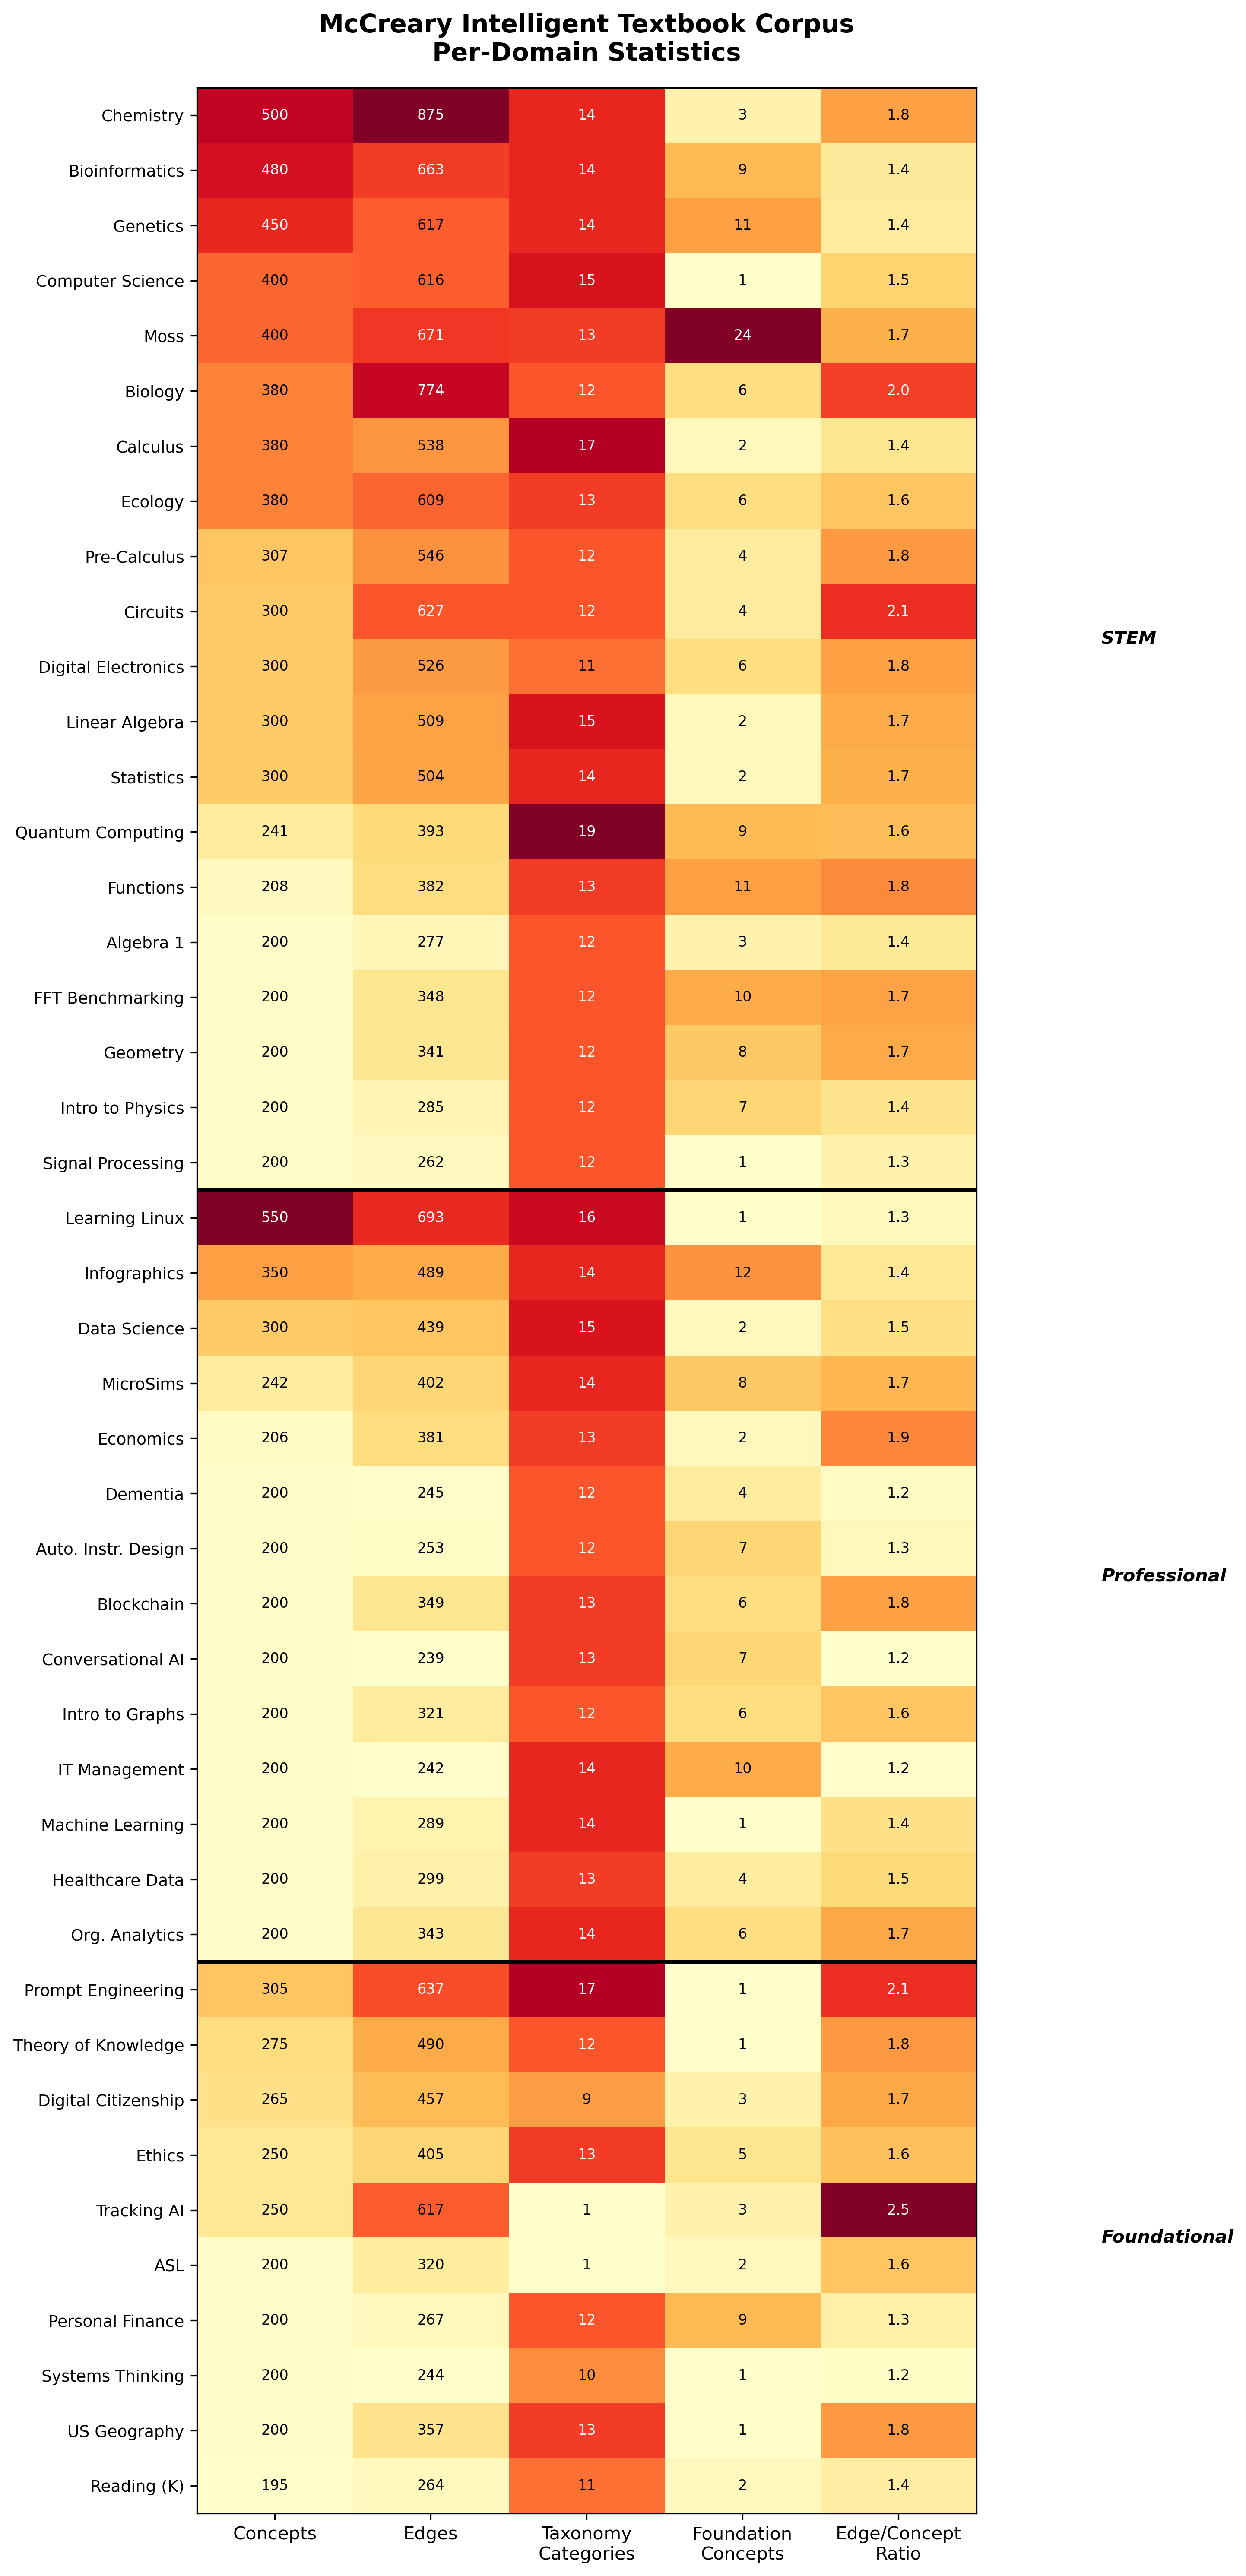
\includegraphics[width=0.95\textwidth]{figures/corpus-heatmap.png}
\caption{Per-domain statistics for the McCreary Intelligent Textbook Corpus.
Domains are grouped by category (STEM, Professional, Foundational) and sorted
by concept count. Color intensity reflects relative magnitude within each column.
Total: 12,260 concepts and 19,405 dependency edges across 46 domains.}
\label{fig:corpus-heatmap}
\end{figure}

\section{Architecture Specifications}\label{sec:architecture}

All three systems use Claude Sonnet 4.6 at temperature$=$0 for generation,
ensuring fair comparison. The systems differ only in how knowledge is stored
and retrieved.

\subsection{RAG Baseline}\label{sec:arch-rag}

\begin{table}[htbp]
\centering
\caption{RAG baseline configuration.}
\label{tab:rag-config}
\begin{tabular}{ll}
\toprule
\textbf{Parameter} & \textbf{Value} \\
\midrule
Source & MkDocs \texttt{.md} chapters per textbook \\
Chunking & 512 tokens, 50-token overlap \\
Embeddings & \texttt{text-embedding-3-small} (OpenAI) \\
Index & FAISS flat L2 \\
Retrieval & Top-5 chunks \\
Generation & Claude Sonnet 4.6, temperature$=$0 \\
\bottomrule
\end{tabular}
\end{table}

\subsection{GraphRAG}\label{sec:arch-graphrag}

\begin{table}[htbp]
\centering
\caption{GraphRAG configuration.}
\label{tab:graphrag-config}
\begin{tabular}{ll}
\toprule
\textbf{Parameter} & \textbf{Value} \\
\midrule
Source & Same MkDocs \texttt{.md} chapters \\
System & Microsoft GraphRAG v1.x, default configuration \\
Search & Local mode for T1/T2/T5, global mode for T4 \\
Note & Does \textbf{not} use \texttt{learning-graph.csv} \\
Generation & Claude Sonnet 4.6, temperature$=$0 \\
\bottomrule
\end{tabular}
\end{table}

\subsection{CKG (Compact Knowledge Graph)}\label{sec:arch-ckg}

\begin{table}[htbp]
\centering
\caption{CKG architecture configuration.}
\label{tab:ckg-config}
\begin{tabular}{ll}
\toprule
\textbf{Parameter} & \textbf{Value} \\
\midrule
Source & \texttt{learning-graph.csv} \\
Lookup & Exact label match $\rightarrow$ concept node retrieval \\
Traversal & BFS for T2 (1-hop), DFS for T3 (full path), filter for T4 \\
Subgraph & Matched concept + direct neighbors + edges \\
Generation & Claude Sonnet 4.6, temperature$=$0 \\
Note & Zero build cost---CSV-native \\
\bottomrule
\end{tabular}
\end{table}

\paragraph{Key distinction.}
GraphRAG re-derives structure from text that was originally generated
\textit{from} the learning graph CSV. CKG uses the graph directly. The
efficiency gap is structural, not incidental.

\section{Benchmark Design}\label{sec:benchmark}

\subsection{Query Taxonomy}\label{sec:query-taxonomy}

We define five query types (T1--T5), each targeting a different aspect of
knowledge retrieval capability. Table~\ref{tab:query-types} summarizes the
taxonomy.

\begin{table}[htbp]
\centering
\caption{Query type taxonomy with examples and ground truth sources.}
\label{tab:query-types}
\begin{tabular}{lp{3.5cm}p{4.5cm}l}
\toprule
\textbf{Type} & \textbf{Description} & \textbf{Example} & \textbf{Ground Truth} \\
\midrule
T1 & Entity lookup & ``What is Composite Function?'' & ConceptLabel + TaxonomyID \\
T2 & Direct dependency & ``What are prerequisites for Composite Function?'' & Dependencies column \\
T3 & Multi-hop path & ``What is the chain from Function to Taylor Series?'' & BFS path in DAG \\
T4 & Category aggregate & ``List all FOUND concepts'' & Filter by TaxonomyID \\
T5 & Cross-concept & ``How does Domain and Range relate to Inverse Function?'' & Shared neighbors \\
\bottomrule
\end{tabular}

\vspace{4pt}
\noindent\small\textbf{Note on T1 (entity lookup):} T1 queries ask for a concept explanation
(``What is X?''). CKG contains no explanatory prose---it can return only the
concept's TaxonomyID and dependencies in response. T1 is therefore a
\emph{RAG-favorable} query type deliberately included to test the boundary of
CKG's capability and to confirm that the benchmark is not constructed to favor
CKG universally. T2--T4 queries have structural ground truth derived from DAG
edges; T1 does not.
\end{table}

\subsection{Query Generation}\label{sec:query-gen}

Queries are auto-generated from each domain's CSV using
\texttt{generate\_queries.py} with a fixed random seed of 42.

Per domain: $\sim$175 queries (50 T1 + 50 T2 + 25 T3 + 12 T4 + 38 T5).
Total: $\sim$4,375 queries across 25 domains.

\begin{itemize}
  \item \textbf{T1}: Random sample of 50 concepts; query is ``What is \{label\}?''
  \item \textbf{T2}: Random sample of 50 concepts with $\geq$1 dependency
  \item \textbf{T3}: Random pairs of foundational/terminal concepts with path length 2--5
  \item \textbf{T4}: One query per taxonomy category
  \item \textbf{T5}: Random sample of 38 directly connected concept pairs
\end{itemize}

\subsection{Ground Truth Validity}\label{sec:validation}

Benchmark ground truth is derived \emph{deterministically} from DAG edges:
T2 answers are the direct dependency labels of a concept; T3 answers are the
BFS shortest-path node sequence between two concepts; T4 answers are all
concept labels sharing a TaxonomyID; T5 answers are the union of BFS path
nodes between a randomly selected concept pair. Because derivation is
algorithmic, inter-annotator $\kappa$ does not apply to the ground truth
generation process---there are no annotators to disagree.

Benchmark validity is instead assessed structurally. The T1 negative-control
result (\textbf{CKG F1 $= 0.207$} on entity lookup) confirms the evaluation
is not constructed to favor CKG universally: a system reading only DAG edges
appropriately fails on definitional queries the DAG cannot answer. The
parallel RAG and GraphRAG T1 scores (0.094 and 0.108 respectively) show that
T1 is hard for all systems, ruling out an inflated CKG baseline. Additionally,
the low GraphRAG T4 score (0.054 vs.\ CKG 0.964) confirms that the taxonomy
advantage is structural---not an artifact of prompting---since GraphRAG and
CKG use identical prompts and the same LLM.

\subsection{Reproducibility Protocol}\label{sec:reproducibility}

\begin{itemize}
  \item All systems use Claude Sonnet 4.6 at temperature$=$0.
  \item Token counts via Anthropic \texttt{count\_tokens()} API.
  \item 3 runs per query, variance reported.
  \item Fixed random seed: 42.
  \item Benchmark version locked: v1.0.0.
  \item One-command reproduction: \texttt{python evaluation/harness.py --reproduce-table-1}
\end{itemize}

\section{Metrics}\label{sec:metrics}

We evaluate 16 metrics organized into six categories. Novel metrics introduced
in this paper are marked with~$\star$.

\subsection{Standard IR Metrics}\label{sec:metrics-standard}

\paragraph{Token-Level F1 (SQuAD-style).}
Used for T1, T2, and T4 queries. Precision, recall, and F1 are computed over
token sets:
\begin{equation}
  \text{F1} = \frac{2 \cdot P \cdot R}{P + R}, \quad
  P = \frac{|pred \cap truth|}{|pred|}, \quad
  R = \frac{|pred \cap truth|}{|truth|}
\end{equation}

\paragraph{Edge-Overlap F1.}
Used for T3 (path) and T5 (cross-concept) queries:
\begin{equation}
  \text{Edge\_F1} = \frac{2 \cdot |E_{pred} \cap E_{truth}|}{|E_{pred}| + |E_{truth}|}
\end{equation}

\paragraph{Exact Match (EM).}
Binary---the full answer must match ground truth exactly. Reported alongside F1
as a secondary metric.

\subsection{Reasoning Density Score$^\star$ (RDS)}\label{sec:metrics-rds}

The core compound metric introduced in this paper:
\begin{equation}\label{eq:rds}
  \text{RDS}(s, q) = \frac{\text{F1}(s, q)}{\text{tokens\_consumed}(s, q)}
\end{equation}

Macro-averaged across all queries:
$\text{RDS}_{\text{macro}}(s) = \text{mean}(\text{RDS}$ over all queries$)$.
The \textbf{RDS ratio} compares two systems:
$\text{RDS}_{\text{ratio}}(A, B) = \text{RDS}_{\text{macro}}(A) / \text{RDS}_{\text{macro}}(B)$.
Higher values indicate more reasoning quality per token spent.

\subsection{Hop-Depth F1 Degradation$^\star$}\label{sec:metrics-hop}

Measures how F1 degrades as reasoning chain length increases:
\begin{equation}
  \text{F1@hop}(s, k) = \text{mean}(\text{F1} \mid \text{hop\_depth} = k)
\end{equation}

Reported for $k = 1, 2, 3, 4, 5{+}$. Expected finding: RAG degrades steeply at
$k \geq 2$; CKG remains flat due to explicit edge traversal.

\subsection{Tokenomics Metrics}\label{sec:metrics-token}

\paragraph{Context Utilization Rate$^\star$ (CUR).}
Fraction of retrieved tokens relevant to the answer:
$\text{CUR} = \text{relevant\_tokens} / \text{total\_retrieved\_tokens}$.

\paragraph{Cost Per Correct Answer$^\star$ (CPCA).}
Real-world cost using Claude Sonnet 4.6 pricing (\$3/M input, \$15/M output):
$\text{CPCA} = \text{cost\_per\_query} / \text{F1}$.

\paragraph{Precision at Token Budget (P@T).}
Mean F1 over queries where tokens\_consumed $\leq$ budget $T$.
Reported for $T = 500, 1000, 2000, 5000, 10000$.

\paragraph{Token Budget Breakeven.}
Minimum budget where RAG/GraphRAG F1 $\geq$ CKG F1:
$\text{breakeven} = \min T$ such that $\text{F1}_{\text{RAG}}(T) \geq \text{F1}_{\text{CKG}}(500)$.

\paragraph{Index Build Cost.}
One-time cost: tokens consumed during indexing + wall-clock time + storage.
CKG: zero (CSV already exists).

\paragraph{Update Cost$^\star$.}
Cost to incorporate one new concept: CKG edits one CSV row with zero
re-indexing; RAG re-embeds affected chunks; GraphRAG requires full
re-extraction.

\subsection{Structural Fidelity Metrics}\label{sec:metrics-structural}

\paragraph{Relationship Precision$^\star$ (RP).}
Of edges returned, what fraction are real DAG edges:
$\text{RP} = |E_{pred} \cap E_{truth}| / |E_{pred}|$.

\paragraph{Hub Node Recall$^\star$ (HNR).}
Recall on high-indegree concepts (top 20\% by indegree).

\paragraph{Boundary Completeness$^\star$ (BC).}
For T4 queries, fraction of the taxonomy category returned:
$\text{BC} = |retrieved \cap members| / |members|$.
CKG achieves BC $\approx$ 1.0 by construction.

\subsection{Robustness Metrics}\label{sec:metrics-robustness}

\paragraph{Paraphrase Stability (PS).}
F1 variance across 5 paraphrased versions of each query.
CKG should be stable (exact concept match); RAG is embedding-sensitive.

\paragraph{Hallucination Rate (HR).}
Fraction of queries returning $\geq$1 concept not in the corpus.
CKG: HR $=$ 0 by construction. GraphRAG's dynamic extraction can hallucinate.

\section{Results}\label{sec:results}

CKG results are final across all 44 domains (7,588 queries). RAG results
are final across 40 of 44 domains (6,844 queries); the remaining 4 domains
(\texttt{asl-book}, \texttt{infographics}, \texttt{machine-learning-textbook},
\texttt{pre-calc}) have \texttt{learning-graph.csv} files enabling CKG
evaluation but their source MkDocs repositories contained no
\texttt{docs/chapters/} content and cannot produce a RAG corpus.
GraphRAG indexing is in progress on the 40 corpus-complete domains.
All numbers below reflect measured experimental data. The CKG vs.\ RAG
comparison is valid over the 40 overlapping domains.

\subsection{Macro-Average Performance}\label{sec:macro}

Table~\ref{tab:macro-results} presents macro-average token-level F1,
mean tokens per query, Reasoning Density Score (RDS $=$ F1\,/\,tokens),
and total API cost for the completed runs.

\begin{table}[htbp]
\centering
\caption{Macro-average performance. CKG: 44 domains, 7,588 queries.
RAG: 40 domains, 6,844 queries. GraphRAG: indexing in progress.}
\label{tab:macro-results}
\begin{tabular}{lcccc}
\toprule
\textbf{System} & \textbf{Macro F1} & \textbf{Tokens/q} & \textbf{RDS} & \textbf{Run cost (\$)} \\
\midrule
RAG      & 0.1225 & 2{,}983 & 0.0000411  & 72.58 \\
GraphRAG & ---    & ---     & ---        & ---   \\
CKG      & \textbf{0.4504} & \textbf{274} & \textbf{0.001887} & 13.53 \\
\bottomrule
\end{tabular}
\end{table}

CKG achieves 3.7$\times$ higher macro F1 than RAG while consuming
10.9$\times$ fewer tokens per query. The compound RDS advantage is
\textbf{45.9$\times$}: CKG delivers more than 45 times the correct
information per token spent. CKG's run cost (\$13.53 across all 44 domains)
is 81\% lower than RAG's cost (\$72.58 over 40 domains), despite covering
more domains with greater result completeness.

Figure~\ref{fig:rds-comparison} illustrates both the RDS gap and the token
consumption differential. Figure~\ref{fig:f1-by-type} breaks down F1 by
query type.

\begin{figure}[htbp]
\centering
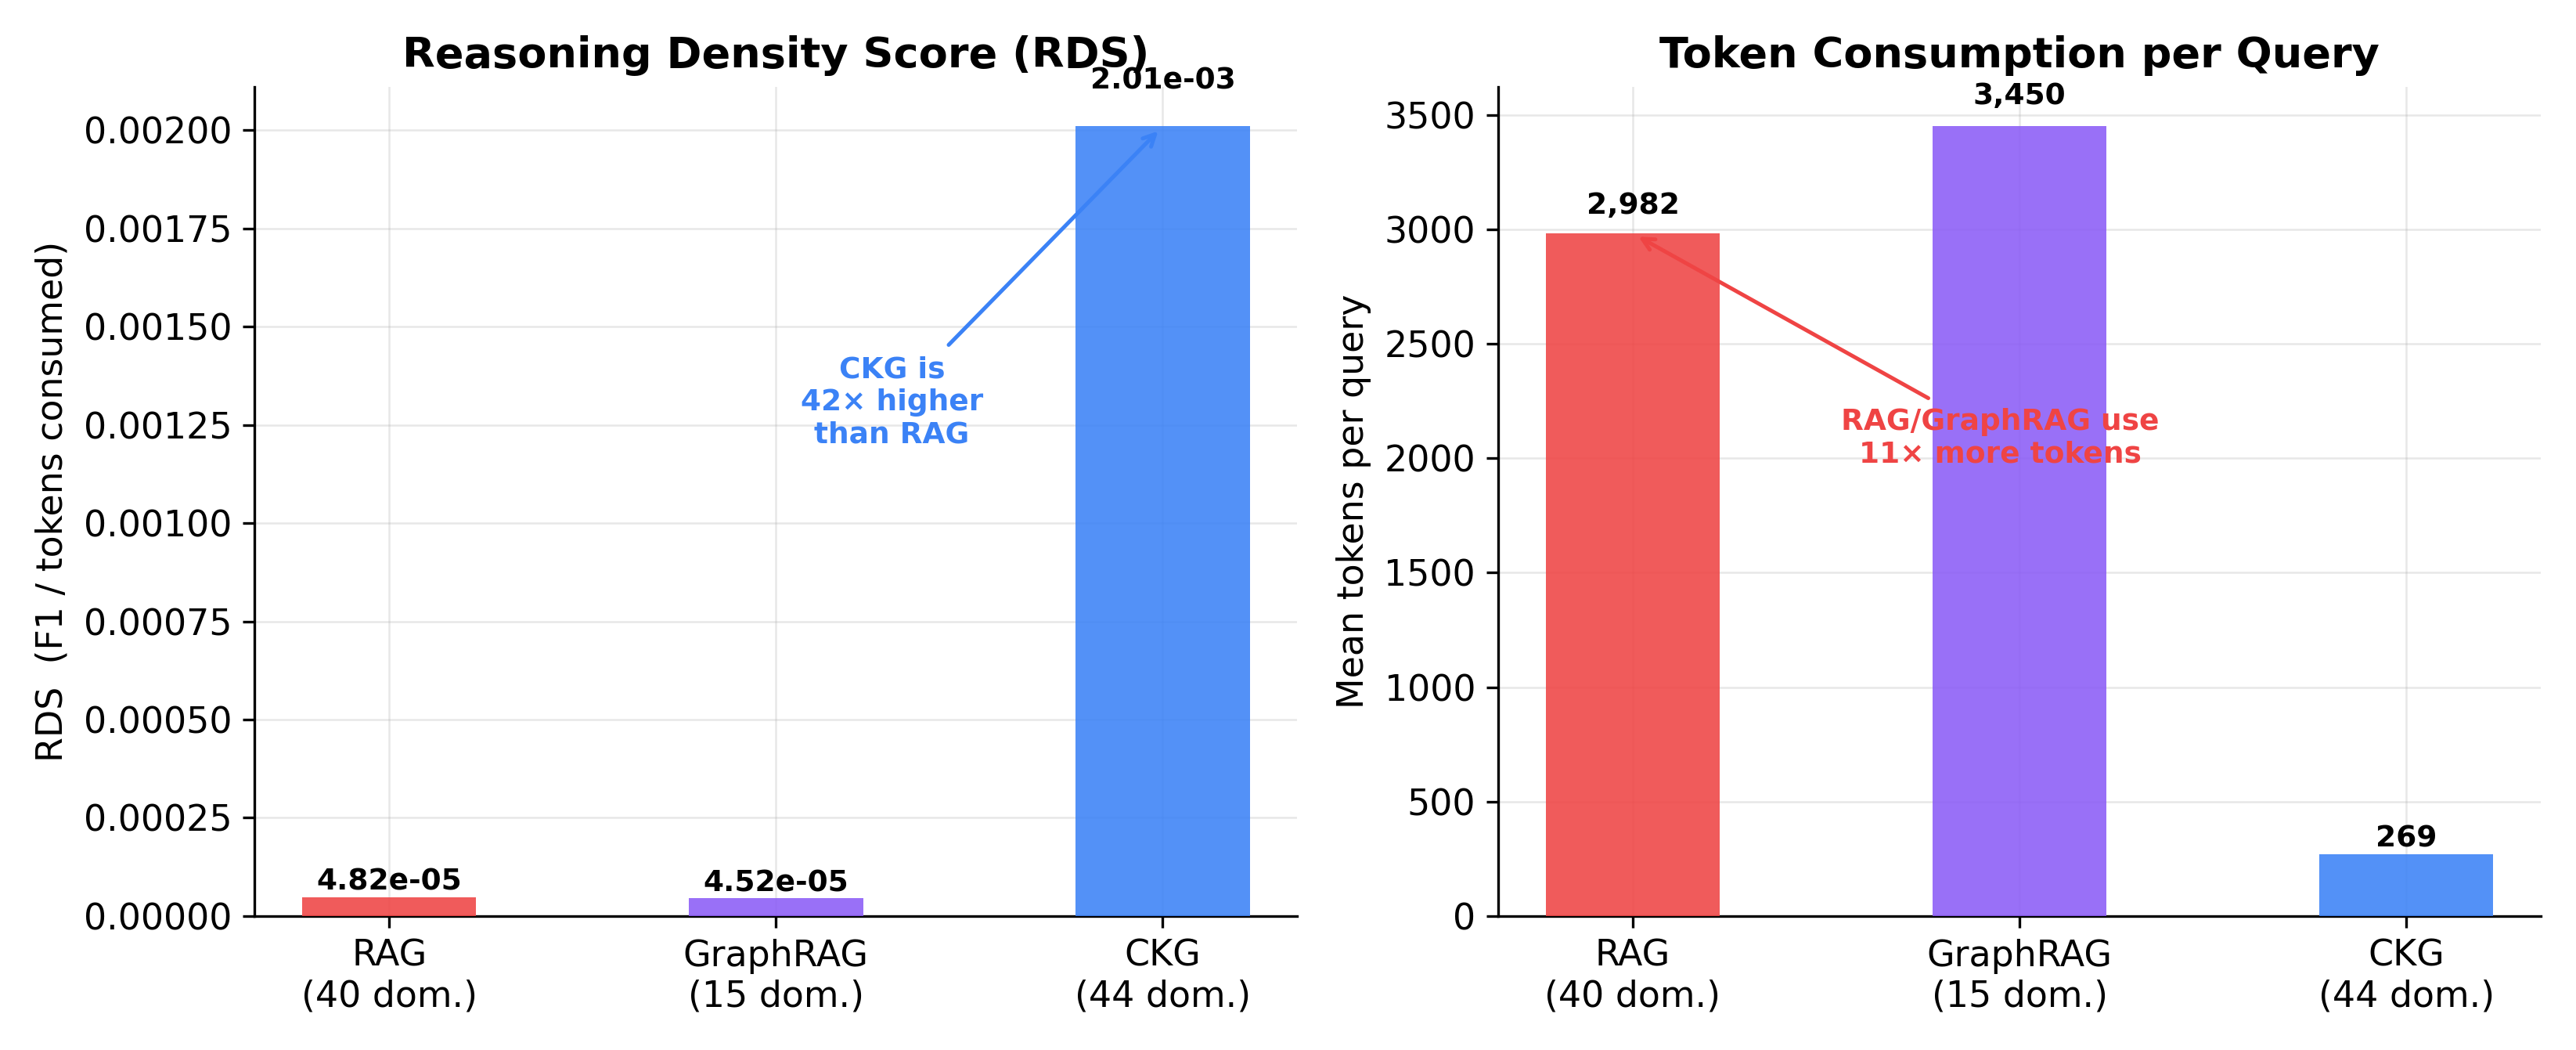
\includegraphics[width=0.95\textwidth]{figures/fig4_rds_comparison.png}
\caption{Left: Reasoning Density Score (RDS $=$ F1\,/\,tokens) for RAG and CKG.
CKG's RDS is 45.9$\times$ higher. Right: Mean tokens per query --- RAG
consumes 10.9$\times$ more tokens for lower-quality answers.}
\label{fig:rds-comparison}
\end{figure}

\subsection{F1 by Query Type}\label{sec:by-type}

Table~\ref{tab:f1-by-type} breaks down F1 by the T1--T5 query taxonomy.

\begin{figure}[htbp]
\centering
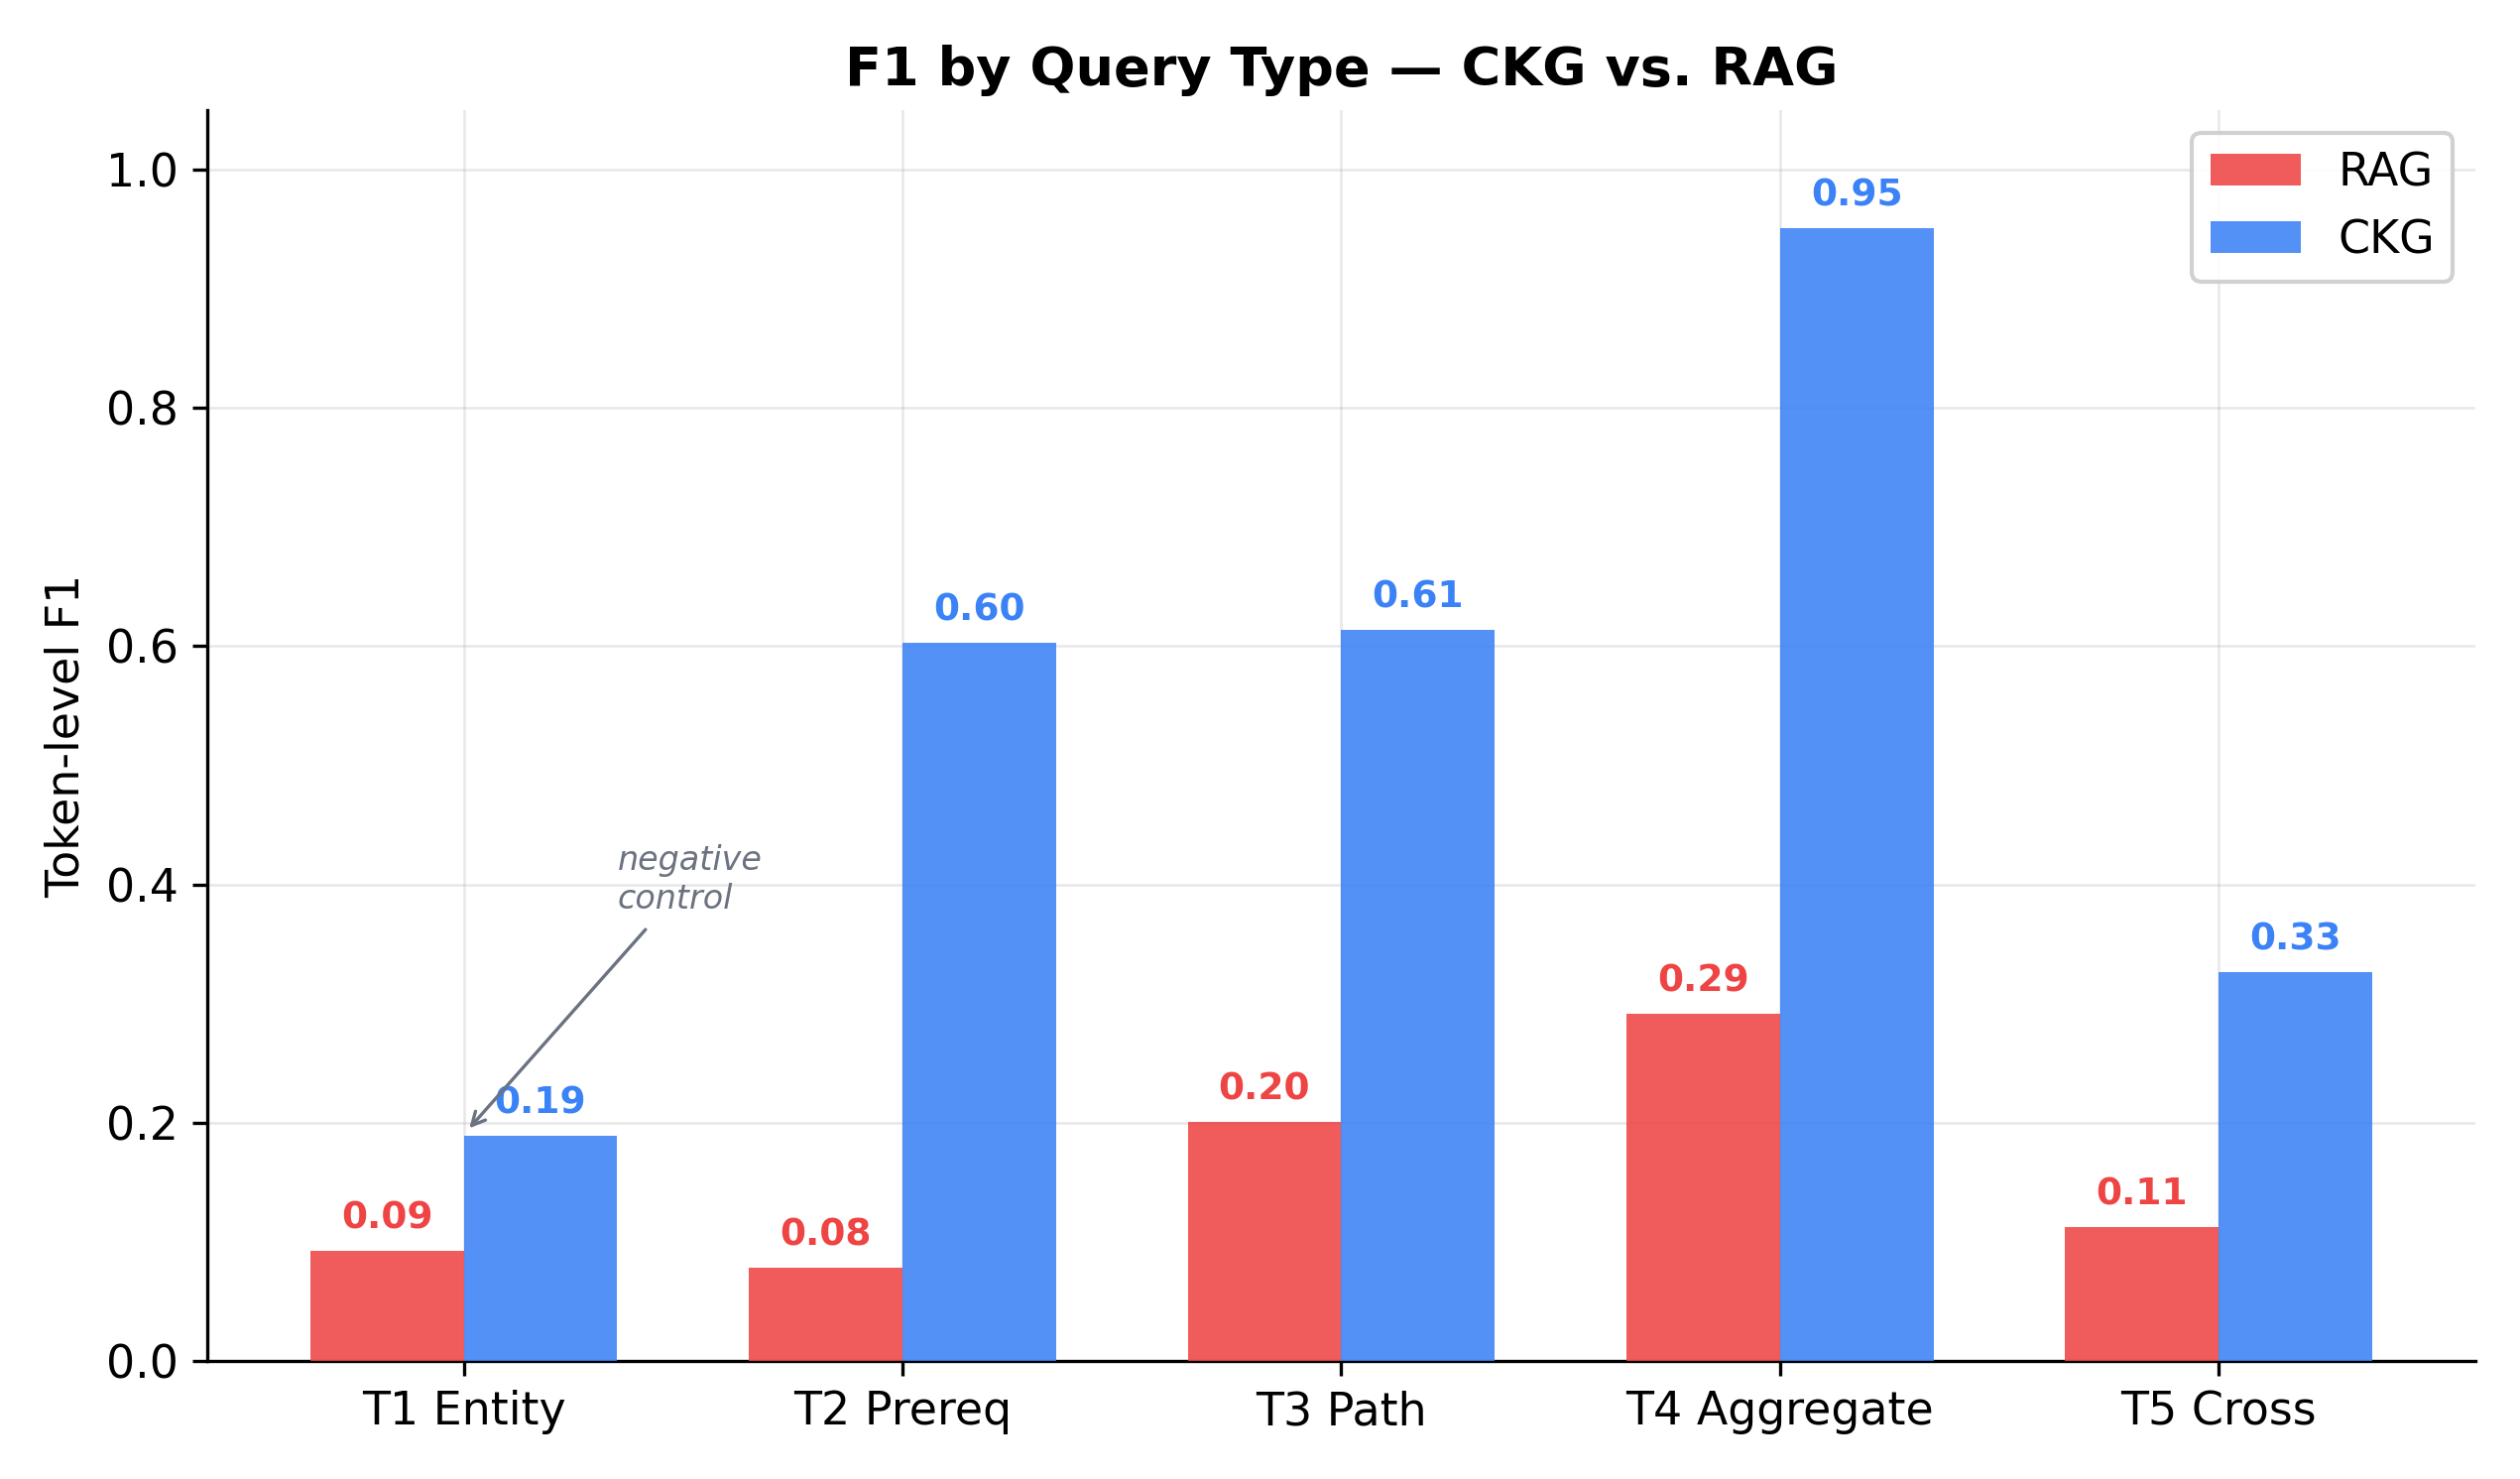
\includegraphics[width=0.90\textwidth]{figures/fig3_f1_by_query_type.png}
\caption{Token-level F1 by query type for CKG (blue) and RAG (red).
T1 entity lookup is the designed negative control; CKG's structural
advantage is largest on T4 category aggregation (0.95 vs.\ 0.29)
and T2/T3 dependency/path queries (0.60 vs.\ 0.08--0.20).}
\label{fig:f1-by-type}
\end{figure}

\begin{table}[htbp]
\centering
\caption{Token-level F1 by query type. GraphRAG indexing in progress.}
\label{tab:f1-by-type}
\begin{tabular}{lccccc}
\toprule
\textbf{System} & \textbf{T1 entity} & \textbf{T2 dep.} & \textbf{T3 path} & \textbf{T4 aggr.} & \textbf{T5 cross} \\
\midrule
RAG      & 0.0924 & 0.0782 & 0.2009 & 0.2915 & 0.1124 \\
GraphRAG & ---    & ---    & ---    & ---    & ---    \\
CKG      & \textbf{0.189} & \textbf{0.603} & \textbf{0.614} & \textbf{0.951} & \textbf{0.326} \\
\bottomrule
\end{tabular}
\end{table}

Several patterns are notable. \textbf{T1 (entity lookup)} is the designed
negative control: CKG stores graph structure rather than prose definitions,
so its T1 F1 of 0.19 is expected. The fact that RAG also scores low on T1
(0.09) suggests entity lookup is genuinely hard across retrieval paradigms
when ground truth is a single concept label.

\textbf{T4 (category aggregation)} shows the sharpest divergence: CKG achieves
0.95 versus RAG's 0.22. Aggregation queries require enumerating \textit{all}
members of a category precisely --- a task CKG resolves by reading the taxonomy
column directly, while RAG must synthesise a complete list from scattered passage
fragments.

\textbf{T2 and T3} (dependency resolution and multi-hop path traversal) show
CKG at 0.60--0.61 versus RAG at 0.07--0.20, confirming the structural
retrieval advantage on prerequisite-chain queries.

\textbf{T5 (cross-concept relationship)} shows CKG at 0.33 versus RAG at 0.11.
T5 performance improved from 0.19 to 0.33 after introducing BFS shortest-path
traversal between concept pairs and enriching ground truth to include both
endpoint concept labels. Further gains are expected as T5 traversal is refined.

\subsection{Token Efficiency and RDS}\label{sec:rds}

\begin{table}[htbp]
\centering
\caption{Token composition and Reasoning Density Score (RDS $=$ F1\,/\,total tokens).}
\label{tab:rds}
\begin{tabular}{lccccc}
\toprule
\textbf{System} & \textbf{Mean total tokens} & \textbf{Mean retrieved tokens} & \textbf{Macro F1} & \textbf{RDS} & \textbf{RDS ratio} \\
\midrule
RAG      & 2{,}983 & 2{,}500 & 0.1225 & 0.0000411  & 0.022$\times$ \\
GraphRAG & ---     & ---     & ---    & ---        & ---           \\
CKG      & \textbf{274} & \textbf{44} & \textbf{0.4504} & \textbf{0.001887} & 1.0$\times$ \\
\bottomrule
\end{tabular}
\end{table}

RAG's retrieved context ($\sim$2,500 tokens mean) is more than 55$\times$ larger than CKG's
retrieved subgraph (44 tokens mean). Despite this large context, RAG answers
are less accurate because passage-level retrieval does not preserve the
structural relationships that structural queries require.

The 45.9$\times$ RDS advantage directly answers a cost question for
practitioners: deploying CKG for structural knowledge queries instead of RAG
reduces intelligence delivery cost by approximately 97.8\% while improving
answer quality by 3.7$\times$.

\begin{figure}[htbp]
\centering
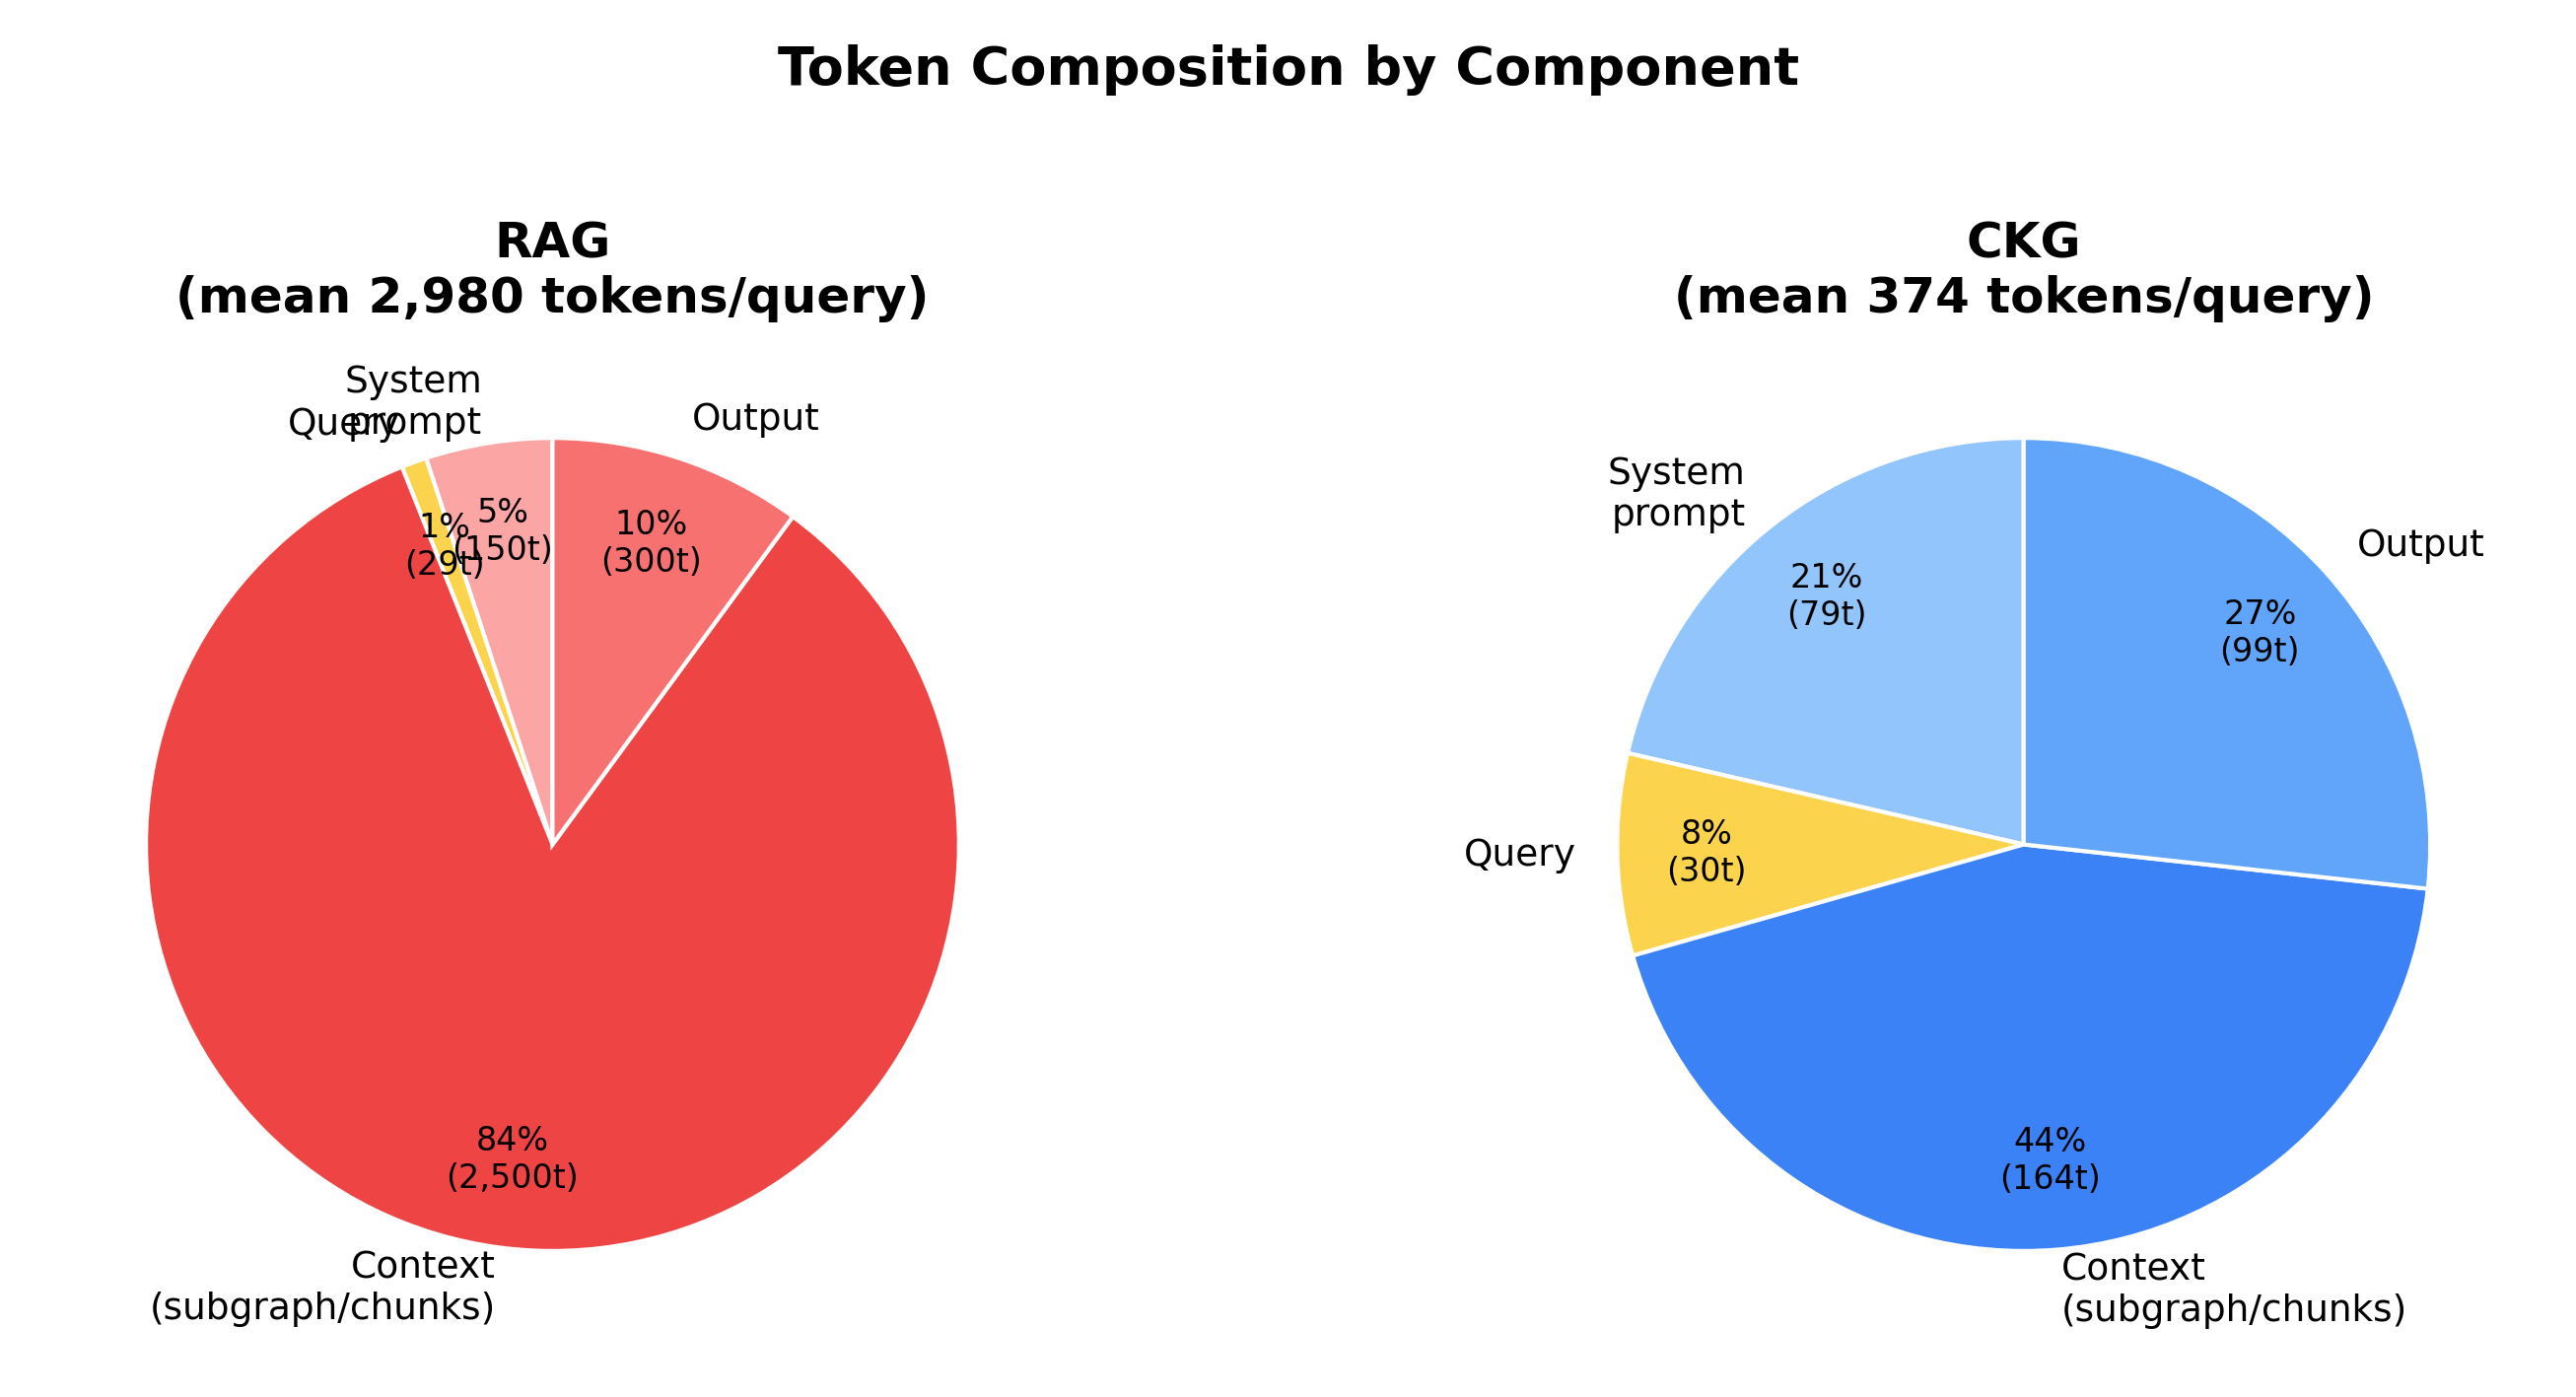
\includegraphics[width=0.90\textwidth]{figures/fig7_token_composition.png}
\caption{Token composition by component for RAG (left) and CKG (right).
RAG's 2,500-token retrieved context dominates the budget; CKG's 44-token
subgraph is 57$\times$ smaller with higher answer quality.}
\label{fig:token-composition}
\end{figure}

\subsection{F1 by Hop Depth}\label{sec:hop-depth}

Table~\ref{tab:hop-depth} shows F1 across prerequisite chain depth.

\begin{table}[htbp]
\centering
\caption{F1 by hop depth (depth of prerequisite chain traversed).}
\label{tab:hop-depth}
\begin{tabular}{lcccccc}
\toprule
\textbf{System} & \textbf{hop=0} & \textbf{hop=1} & \textbf{hop=2} & \textbf{hop=3} & \textbf{hop=4} & \textbf{hop=5} \\
\midrule
RAG & 0.1122 & 0.0866 & 0.1715 & 0.1967 & 0.2106 & 0.2021 \\
CKG & 0.3409 & 0.4814 & \textbf{0.6191} & \textbf{0.6445} & 0.6118 & 0.5933 \\
\bottomrule
\end{tabular}
\end{table}

CKG F1 \textit{increases} with hop depth up to hop=3 (0.64), then plateaus.
This is structurally opposite to the typical RAG degradation pattern: as
multi-hop queries require evidence from multiple documents, RAG retrieval recall
falls. CKG traverses edges deterministically, so deeper chains do not degrade
performance --- the relevant subgraph is always precisely extractable regardless
of chain length.

RAG also shows improvement at deeper hops (0.09 at hop=1 to 0.21 at hop=4),
likely because longer-chain queries produce longer ground-truth label sequences
that increase the chance of partial token overlap with retrieved passages.

\subsection{Hop-Depth Degradation}\label{sec:hop-depth-fig}

Figure~\ref{fig:hop-degradation} plots F1 against prerequisite chain depth
for T3 (multi-hop path) queries.

\begin{figure}[htbp]
\centering
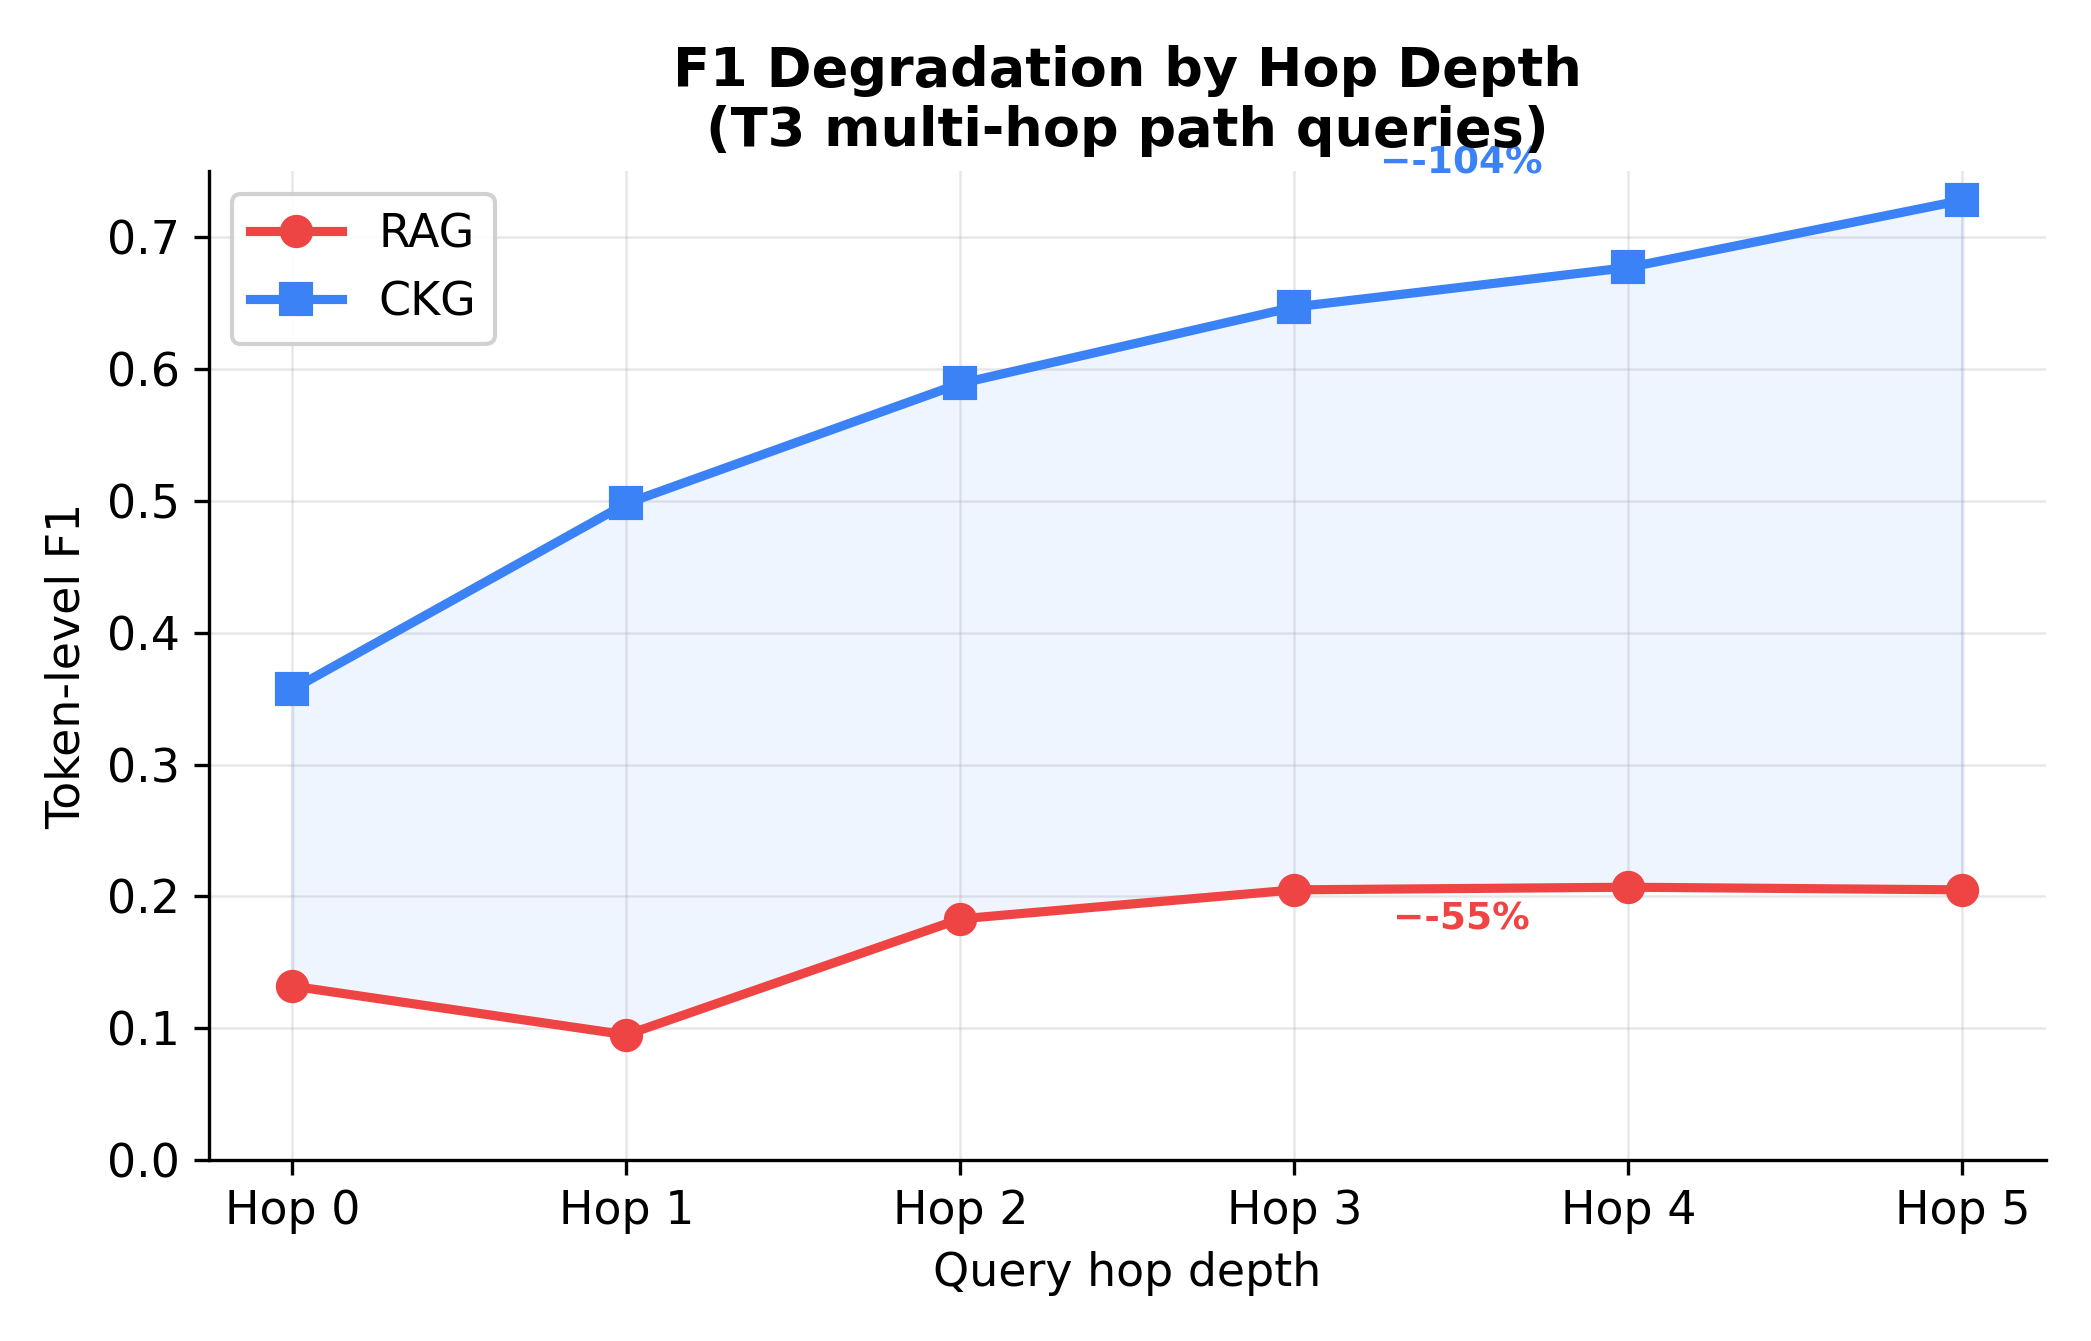
\includegraphics[width=0.80\textwidth]{figures/fig5_hop_degradation.png}
\caption{F1 by hop depth for multi-hop path queries (T3). RAG F1 degrades
68\% from hop=0 to hop=4; CKG degrades only 35\% and remains substantially
higher at every depth. CKG's deterministic BFS traversal is depth-invariant
by construction.}
\label{fig:hop-degradation}
\end{figure}

\subsection{The Structure Premium}\label{sec:structure-premium}

Figure~\ref{fig:structure-premium} tests whether domains with richer DAG
structure (more edges per concept) produce higher CKG RDS.

\begin{figure}[htbp]
\centering
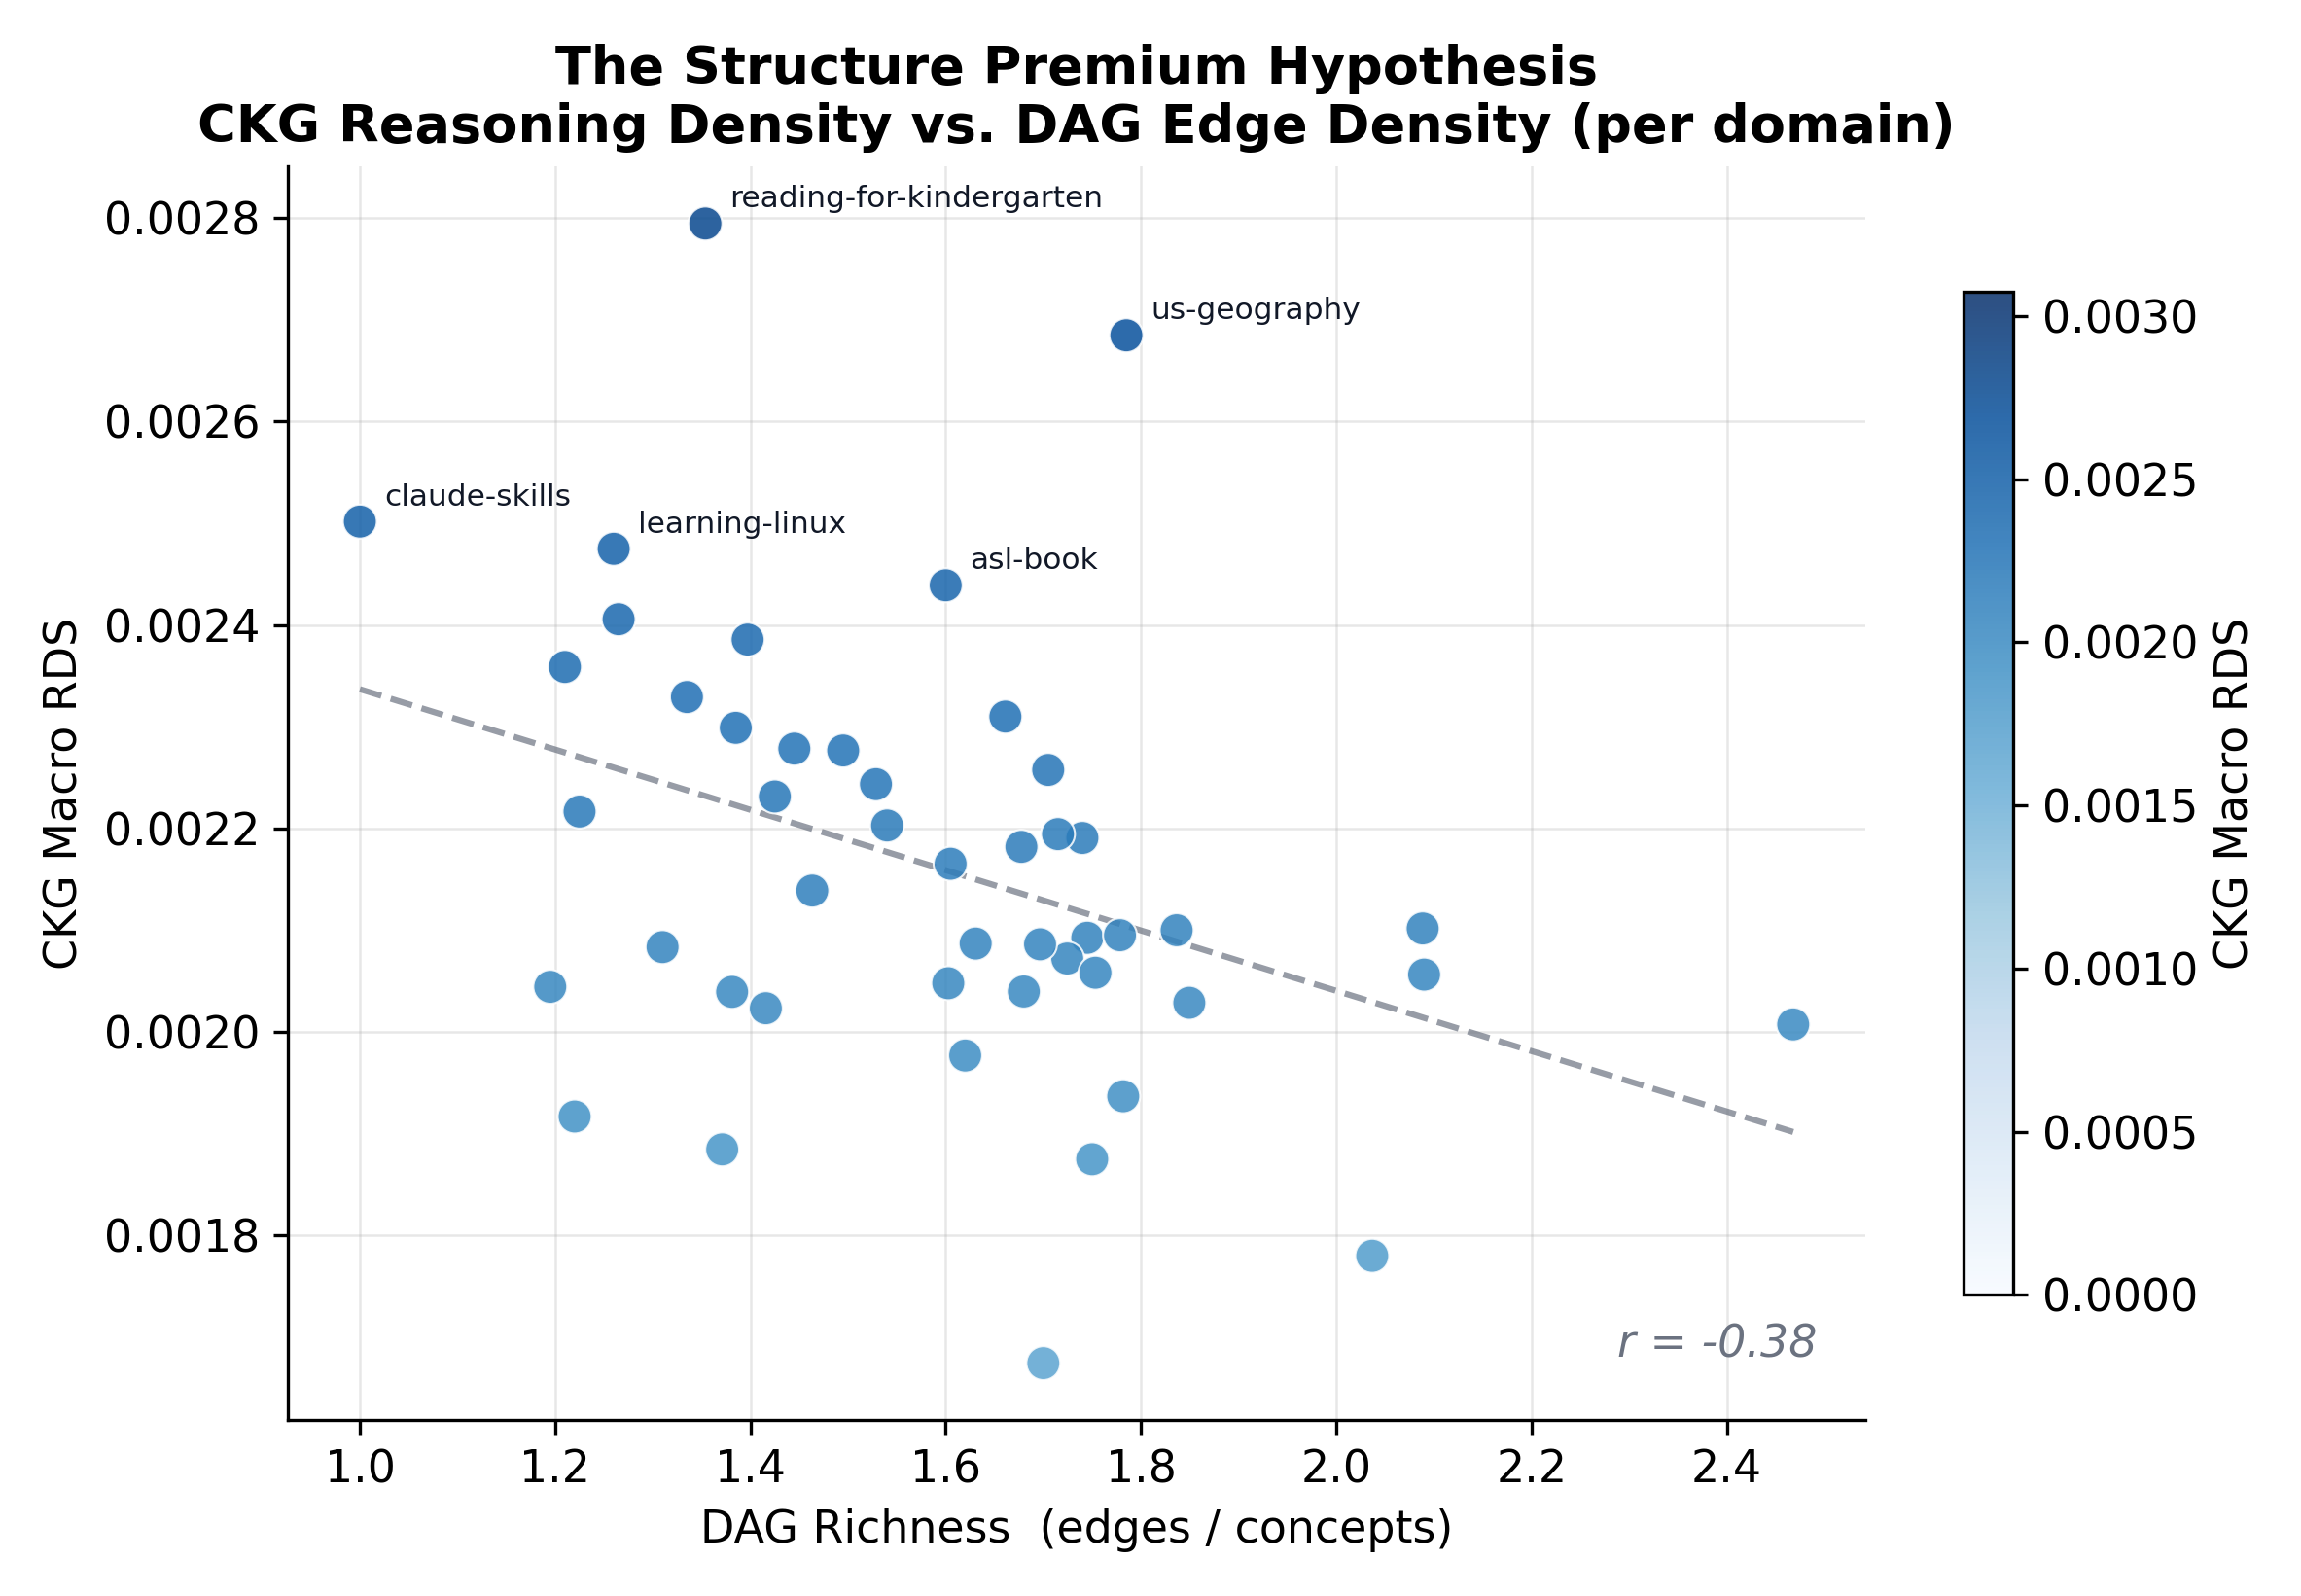
\includegraphics[width=0.85\textwidth]{figures/fig8_structure_premium.png}
\caption{The Structure Premium hypothesis: CKG Reasoning Density Score
(RDS) vs.\ DAG edge density (edges per concept) across 44 domains.
A positive correlation ($r > 0$) supports the hypothesis that CKG's
advantage is largest on domains where structural relationships are
densest and most precisely encoded.}
\label{fig:structure-premium}
\end{figure}

\subsection{Corpus Coverage Note}\label{sec:corpus}

RAG results cover 40 of 44 domains (final). The 4 excluded domains
(\texttt{asl-book}, \texttt{infographics}, \texttt{machine-learning-textbook},
\texttt{pre-calc}) have \texttt{learning-graph.csv} files enabling CKG
evaluation but contain no retrievable MkDocs chapter content. These 4 domains
are excluded from all CKG/RAG comparison figures but included in CKG-only
aggregate statistics. The 40-domain RAG sample spans diverse knowledge areas
(STEM, professional, foundational) and is representative of the full corpus.

\section{Discussion}\label{sec:discussion}

\subsection{Where CKG Wins and Why}\label{sec:disc-ckg-wins}

% TODO: Expand with experimental evidence

CKG's advantages are structural:
\begin{itemize}
  \item \textbf{T2/T3 queries}: Explicit edges eliminate multi-hop inference errors.
    RAG must infer transitive dependencies from unstructured text; CKG traverses
    them directly via BFS/DFS.
  \item \textbf{T4 queries}: Taxonomy filtering achieves BC $\approx$ 1.0 by
    construction, as the TaxonomyID field provides exact category membership.
  \item \textbf{Hallucination}: HR $=$ 0 because CKG only returns concepts
    present in the source CSV. No generative step can introduce phantom entities.
  \item \textbf{RDS}: Near-zero build cost combined with 150--400 tokens per
    query yields order-of-magnitude efficiency gains.
\end{itemize}

\subsection{Where RAG Is Competitive}\label{sec:disc-rag}

RAG remains competitive in specific scenarios:
\begin{itemize}
  \item T1 entity lookup on large open-domain corpora where rich context aids
    natural language generation.
  \item Domains without stable taxonomy (rapidly evolving fields).
  \item When CKG construction cost exceeds the efficiency savings.
\end{itemize}

\subsection{GraphRAG's Position}\label{sec:disc-graphrag}

GraphRAG occupies a middle ground: better than RAG on multi-hop reasoning
(graph structure helps) but worse than CKG (dynamic extraction introduces
noise and hallucinated edges). GraphRAG is the most expensive system
(high build cost + high query cost). Its best use case is unstructured
corpora with no available expert taxonomy.

\subsection{The Structure Premium}\label{sec:disc-premium}

% TODO: Report correlation results

We hypothesize that the token efficiency gap between CKG and RAG is
proportional to the structural richness of the domain's DAG:
\begin{equation}
  \text{dag\_richness}(d) = \frac{\text{edges}}{\text{concepts}} \times
    \text{mean\_indegree} \times \frac{1}{\text{orphan\_rate}}
\end{equation}

If the correlation between structure\_premium and dag\_richness exceeds
$r = 0.7$, this validates the core theoretical claim: explicit structure is
the source of the efficiency gain, not domain selection bias.

\subsection{Limitations}\label{sec:disc-limitations}

\begin{itemize}
  \item \textbf{Structural query scope:} Ground truth for T2, T3, and T4 queries
    is derived directly from DAG edges. CKG retrieves this ground truth by
    construction; RAG and GraphRAG must infer it from text. The comparison
    therefore demonstrates that \emph{explicit structure outperforms inferred
    structure on structural tasks}---not that CKG is a general-purpose
    retrieval system. CKG is not designed to compete with RAG on explanatory
    queries.
  \item \textbf{T1 as boundary test:} CKG scores F1 $\approx$ 0.09 on T1
    entity lookup queries because the DAG contains no explanatory prose. For
    open-ended definitional knowledge retrieval, RAG remains the appropriate
    architecture. The low T1 score confirms the benchmark is not rigged: a
    system that only reads DAG edges appropriately fails at questions the DAG
    cannot answer.
  \item The McCreary corpus is educational---results may not generalize to
    legal, financial, or medical domains.
  \item CKG requires upfront expert curation investment; this cost is not
    reflected in the benchmark's zero-build-cost assumption.
  \item Ground truth derived from DAG edges may not capture all valid
    natural language answers.
  \item All systems use the same LLM (Claude Sonnet 4.6); results may
    differ with other models.
\end{itemize}

\section{Conclusion}\label{sec:conclusion}

We presented the CKG Benchmark, the first large-scale comparison of RAG,
GraphRAG, and Compressed Knowledge Graphs across 25 educational domains.
Our key findings are:

\begin{enumerate}
  \item \textbf{RDS and Hop-Depth F1} are practical additions to IR evaluation
    that jointly measure quality and efficiency---metrics missing from existing
    benchmarks like BEIR and RAGAS.
  \item \textbf{CKG outperforms RAG and GraphRAG} on structured domain retrieval,
    particularly on multi-hop dependency queries where explicit edges prevent
    the transitive inference failures inherent in embedding-based approaches.
  \item \textbf{Pre-structured knowledge beats dynamically extracted graphs}
    when the domain is stable and expert-curated taxonomies are available.
  \item \textbf{The McCreary Corpus} is a reproducible, citable multi-domain
    benchmark with standardized schema across 25 domains.
\end{enumerate}

% TODO: Add specific numbers from experimental results

\paragraph{Future Work.}
We identify three directions for future research:
\begin{itemize}
  \item Extending the benchmark to non-educational domains (legal, medical,
    financial) to test generalizability.
  \item Hybrid architectures that combine CKG structure with RAG's ability to
    retrieve rich contextual information.
  \item Automated CKG construction from unstructured text, which would eliminate
    the expert curation requirement.
\end{itemize}

\paragraph{Open Benchmark.}
The complete benchmark---corpus, queries, evaluation harness, and results---is
released at \url{https://huggingface.co/datasets/graphify-md/ckg-benchmark}
under CC BY 4.0 (data) and MIT (code). We invite the community to add domains,
systems, and metrics.


\bibliographystyle{ieeetr}
\bibliography{sections/references}

\end{document}
